% ============================================================
%  第九章 极化子理论（§1–§5 + 章末参考文献）
%  底本：高等教育出版社《固体理论》第二版；原书印刷页 343–368
%  （PDF 页 = 印刷页 + 20）
%  公式编号自检：§1 (9.1.1)–(9.1.2)；§2 (9.2.1)–(9.2.9)；
%    §3 (9.3.1)–(9.3.50)；§4 (9.4.1)–(9.4.61)；
%    §5 (9.5.1)–(9.5.26)。全章自动编号 148 个，无缺号
%    （任务单 tags=146 系 (9.3.24) 无 tag、(9.4.32) 编号嵌于式内
%    未被脚本计入所致）。
%
%  任务单所列"缺号"逐条对照原书页面判定（均非原书跳号）：
%    (9.3.12) OCR tag 残缺（".3.12"），原书 p347 在号；
%    (9.3.23)(9.3.24) OCR 把 ℋ̄₀ 的跨页两块并入一号、ℋ̄₁ 只剩游离
%             的"(9.3.24)"文字，已按 p348–349 拆为两式；
%    (9.3.47) OCR tag 残缺（".47"），原书 p352 在号；
%    (9.4.32) 编号嵌在式内（p359），已归还本式；
%    (9.4.54) OCR tag 残缺（p362），原书在号；
%    (9.5.9)  编号残缺为"(9.5."（p365），原书在号。
%
%  已修正的 OCR/原书错误（除全角句点转"."、删 ~ 间隔符、收紧
%  \mathrm{d}、拆开行内公式与中文、上标 [N] 转正文等常规项外）：
%  1. §3 章首段 OCR"表象在 P_op 其中"语序错乱，按 p346 复原为
%     "适合的表象在其中总动量算符变为 c 数"；"为了求得"后按原书补 ℋ；
%     "可 j^μ 格求得"→"可严格求得"（p349）。
%  2. (9.3.7) OCR"\Ddot{H}"→ℋ，全章花体 ℋ、ℰ₀、ℰ 统一 \mathscr；
%     < < A | B > > 类括号统一 \langle…\rangle。
%  3. 原书 p346 (9.3.9) 前脚注①"更确切地说，这时可将波函数写成
%     Ψ=e^{iP·r/ħ}Ψ₁，式(9.3.7)自动变为式(9.3.9)."OCR 漏失，
%     已按页脚补录。
%  4. 原书 p348 (9.3.23) 首项"P-Σ_q a_q⁺a_q ħq²"→ ħq（量纲；
%     与 (9.3.9) 及同式内 (ħ²/m)q·q' 项一致）。
%  5. 原书 p349 (9.3.25) 第三项"ħ/2m(Σ_q q|f(q)|²)²"→ ħ²/2m
%     （与 (9.3.23) 同一来源项 ħ²/2m[Σ_q|f(q)|²q]² 一致，量纲）。
%  6. "李政道等人等经数值计算"→"李政道等人经数值计算"（p351 衍字）。
%  7. (9.3.44)(9.3.46) 中 OCR 乱码（a_{q⁺}⁺ 等）按 p351–352 复原。
%  8. 原书 p362 (9.4.51) "φ(0)=iΣ_q|λ_q|²[...]^{1/2}"→ 2Σ_q…
%     （i 为 2 之误：与 (9.4.50) 于 z=0 取值及 (9.4.54) 首行
%     2S_T-φ(0) 的展开一致）。
%  9. 原书 p362 (9.4.53) 首行被积函数"e^{φ(T)}"→ e^{φ(z)}
%     （回路积分变量为 z，见 (9.4.50)）。
% 10. (9.4.46) 整块 OCR 乱码按 p361 复原；(9.4.30)(9.4.31) OCR
%     拆块按 p358–359 原书两号照排；(9.4.20) Σ_ρ 上的撇号照原书。
% 11. (9.5.5) OCR 漏首项负号，按 p364 补"-ħ²/(2m)·d²/dx²"。
% 12. (9.5.10) 求和指标 OCR 作 n，按 p365 原书 Σ_m 复原。
% 13. §5 末段"聚Z炔"→"聚乙炔"（p367）；"关系19]"→"关系[19]"
%     （p363）；TiO₂ 的 0→O（p363）。
% 14. 文献[2]"Pines D. Kuper"→"Pines D, Kuper C G"（p367 逗号）。
%  插图：本章仅 1 图——图 9.1 f(α) 曲线（原书印刷 p353/PDF p373）。
%  任务单所称"图 9.1–9.6 共 6 幅"与原书不符：已逐页核对 PDF
%  p363–389（印刷 343–369），本章只有图 9.1，其余页无插图
%  （PDF p389 起已是第十章）。
%  遗留问题：
%  · 图 9.1 为占位图（figures/fig9-1.pdf），待重绘代理按原书绘制；
%  · (9.4.29) 原书印 e^{+ik·ρ}，而 (9.4.27)(9.4.37)(9.4.40) 印
%    e^{-ik·ρ}，照录未改；
%  · (9.5.9) 原书左端作"i∂/∂t"（无 ħ），与 (9.5.7) 不一致，系原书
%    照排，未改；(9.3.25)→(9.3.31) 的中间代数照录，未作改写。
% ============================================================
\chapter{极化子理论}

\section{大极化子与小极化子}

本章研究离子晶体中一个缓慢运动电子的特性.由于运动电子的库仑势，将使周围晶格极化，正离子被吸向电子，负离子被斥向外移.这一正、负离子的相对位移，形成一个围绕电子的极化场.这个场反过来作用于电子，改变电子的能量与状态，并伴随着电子在晶格中运动.因此，电子与它周围的极化场构成一个互作用的整体，称为极化子.离子晶体中导带底部的电子或价带顶部的空穴都带着周围的极化场运动，载流子实际上都是极化子.由此可见，极化子是离子晶体中的基本载流子，极化子的研究对于解释离子晶体和极性半导体中的光跃迁过程及输运现象有重要意义.

极化子的尺寸可由电子（或空穴）周围晶格畸变区域的大小决定.当这个区域比晶格常数大得多时称为大极化子，这时离子晶体可以当连续介质处理.当电子周围的晶格畸变区小于或等于晶格常数量级时，必须考虑晶体结构的原子性，并用晶格模型处理极化子问题，这就是小极化子情况.

从场论角度讲，极化子是慢电子与光学模纵声子（LO声子）相互作用系统的准粒子.正如第五章§4中分析所指出，上述晶格畸变可解释为电子在其周围激发LO虚声子.由此不难利用测不准关系式对极化子的尺寸作如下简单估计：设 $\hbar\omega_{\mathrm L}$ 为LO声量子，则电子发射或吸收LO声子将产生能量的不确定性：
\begin{equation}
  \Delta E=\hbar\omega_{\mathrm L}
\end{equation}
考虑到 $E=\dfrac{\hbar^{2}k^{2}}{2m}$，m为能带电子的有效质量，则对原为静止的电子，当吸收一个LO虚声子后波数的不确定度为 $\Delta k=(2m\omega_{\mathrm L}/\hbar)^{\frac{1}{2}}$，由此求得位置的不确定度
\begin{equation}
  \Delta r=\frac{1}{\Delta k}
  =\Bigl(\frac{\hbar}{2m\omega_{\mathrm L}}\Bigr)^{\frac{1}{2}}
\end{equation}
对于多数的离子晶体，例如碱金属的卤化物其能带电子的有效质量可近似取自由电子质量，算出的 $\Delta r\approx 1\,\mathrm{nm}$ 略大于晶格常数.对于极性半导体，如Ⅱ-Ⅵ和Ⅲ-Ⅴ族化合物能带电子的有效质量比自由电子质量小100倍，极化子的尺寸约为10nm，远大于晶格常数，在这些材料中载流子是大极化子.对于窄带半导体如NiO，能带电子的有效质量较大，$\Delta r$ 小于或等于晶格常数，属于小极化子情况.

若计入电子与LO声子的互作用，则有效质量将随耦合强度增加而增大，相应的极化子尺寸会随之减小，因此小极化子在窄带与强耦合情况下出现，这时电子被自己感生的极化场所束缚，在格点附近形成了局域态，朗道称其为电子的自陷态.小极化子在晶格中运动的迁移率很小，必须依靠热声子的激活才能跳到邻近的格点上去，从而形成新格点上的局域态.这是小极化子导电的特征，它与离子晶体中空位电导的机制相似.

下面将首先引入大极化子的哈密顿量（§2），然后研究中间耦合强度的大极化子能谱（§3），最后介绍小极化理论（§4）和准一维系统中的极化子解（§5）.

\section{大极化子的弗留里希哈密顿量}

极化子的哈密顿量由三部分组成：
\begin{equation}
  H=H_{\mathrm e}+H_{\mathrm p}+H_{\mathrm{int}}
\end{equation}
$H_{\mathrm e}$ 包括电子的动能和电子在晶格周期场中的势能，利用有效质量近似可将导带中慢电子的哈密顿量写为
\begin{equation}
  H_{\mathrm e}=p^{2}/2m
\end{equation}
m 应理解为能带电子的有效质量. $H_{\mathrm p}$ 代表LO声子的哈密顿量
\begin{equation}
  H_{\mathrm p}=\sum_{q}\hbar\omega_{\mathrm L}a_{q}^{+}a_{q}
\end{equation}
其中 $a_{q}^{+}$ 与 $a_{q}$ 是LO声子的产生及消灭算符，满足玻色子对易式. $H_{\mathrm{int}}$ 是单个电子与晶格极化场之间的互作用势能.对于大极化子可以采用连续模型按黄昆方程定出（见第五章§4）
\begin{equation}
\begin{aligned}
  &H_{\mathrm{int}}=-e\phi(\boldsymbol{r})\\
  &\phi(\boldsymbol{r})=-\mathrm{i}4\pi F
  \sum_{q}\frac{1}{q}\bigl(a_{q}\mathrm{e}^{\mathrm{i}\boldsymbol{q}\cdot\boldsymbol{r}}
  -a_{q}^{+}\mathrm{e}^{-\mathrm{i}\boldsymbol{q}\cdot\boldsymbol{r}}\bigr)\\
  &F=\biggl\{\frac{\hbar\omega_{\mathrm L}}{8\pi}
  \biggl(\frac{1}{\varepsilon_{\infty}}-\frac{1}{\varepsilon_{0}}\biggr)\biggr\}^{\frac{1}{2}}
\end{aligned}
\end{equation}
这里 $\varepsilon_{0}$ 为静态介电常数，$\varepsilon_{\infty}$ 为高频介电常数，$\boldsymbol{r}$ 为电子坐标，$\omega_{\mathrm L}$ 为LO声子频率，可取为常数.式(9.2.4)实际上就是单个电子与LO声子的相互作用的哈密顿量.为了今后计算方便，我们采用李政道、勒欧和派因斯\textsuperscript{[1]}（Lee-Low-Pines，以后简称LLP）的记号，将 $H_{\mathrm{int}}$ 写为
\begin{equation}
  H_{\mathrm{int}}=\sum_{q}\bigl(V_{q}a_{q}\mathrm{e}^{\mathrm{i}\boldsymbol{q}\cdot\boldsymbol{r}}
  +V_{q}^{+}a_{q}^{+}\mathrm{e}^{-\mathrm{i}\boldsymbol{q}\cdot\boldsymbol{r}}\bigr)
\end{equation}
其中
\begin{equation}
  V_{q}\equiv\mathrm{i}\,\frac{4\pi eF}{q}
  =\mathrm{i}\,\frac{\hbar\omega_{\mathrm L}}{q}
  \biggl(\frac{\hbar}{2m\omega_{\mathrm L}}\biggr)^{\frac{1}{4}}
  (4\pi\alpha)^{\frac{1}{2}}
\end{equation}
\begin{equation}
  \alpha=\frac{e^{2}}{2\hbar\omega_{\mathrm L}}
  \biggl(\frac{2m\omega_{\mathrm L}}{\hbar}\biggr)^{\frac{1}{2}}
  \biggl(\frac{1}{\varepsilon_{\infty}}-\frac{1}{\varepsilon_{0}}\biggr)
\end{equation}
$\alpha$ 是量纲为1的耦合常数，在这里样品取单位体积.

综合式(9.2.2)、(9.2.3)与(9.2.5)求得大极化子的哈密顿量为
\begin{equation}
  H=\frac{p^{2}}{2m}+\sum_{q}\hbar\omega_{\mathrm L}a_{q}^{+}a_{q}
  +\sum_{q}\bigl(V_{q}a_{q}\mathrm{e}^{\mathrm{i}\boldsymbol{q}\cdot\boldsymbol{r}}+h.c.\bigr)
\end{equation}
在第五章§4中我们曾经用微扰方法计算了 $T=0$ K时极化子的能谱，求得
\begin{equation}
\left.
\begin{aligned}
  &E_{k}=-\alpha\hbar\omega_{\mathrm L}
  +\frac{\hbar^{2}k^{2}}{2m^{*}}\\
  &m^{*}=\frac{m}{1-\dfrac{\alpha}{6}}
\end{aligned}\right\}
\end{equation}
所用的方法只适用于弱耦合 $\left(\alpha\ll1\right)$ 情况，但是大多数离子晶体的耦合常数在3到6之间，对于这些材料由于电子与LO声子之间耦合较强，微扰方法失效，必须采用非微扰近似处理，这是极化子理论的基本问题.

\section{\texorpdfstring{LLP中间耦合理论\textsuperscript{[2]}}{LLP中间耦合理论[2]}}

计算大极化子自能的代表性工作是李政道等人的正则变换方法\textsuperscript{[1]}，它适用于 $\alpha<6$ 的中间耦合强度情况.

\subsection*{1. 消去电子坐标的正则变换}

由于存在电子-声子互作用，电子的动量 $\boldsymbol{p}=\dfrac{\hbar}{\mathrm{i}}\boldsymbol{\nabla}$ 不再是运动积分.如果计入声子动量并引入系统的总动量算符
\begin{equation}
  \boldsymbol{P}_{\mathrm{op}}=\boldsymbol{p}
  +\sum_{q}\hbar\boldsymbol{q}\,a_{q}^{+}a_{q}
\end{equation}
则不难验证 $\boldsymbol{P}_{\mathrm{op}}$ 与极化子的哈密顿量H［见式(9.2.8)］对易
\begin{equation}
  \left[H,\boldsymbol{P}_{\mathrm{op}}\right]=0
\end{equation}
因此 $\boldsymbol{P}_{\mathrm{op}}$ 是运动积分.这说明通过正则变换可以找到一个适合的表象在其中总动量算符变为c数，而哈密顿量中不再包含电子的坐标.李政道等人考虑正则变换
\begin{equation}
\begin{aligned}
  &\varPhi=U_{1}\varPsi\\
  &\boldsymbol{U}_{1}=\exp\Bigl(-\mathrm{i}\sum_{q}a_{q}^{+}a_{q}\,
  \boldsymbol{q}\cdot\boldsymbol{r}\Bigr)
\end{aligned}
\end{equation}
这里 $\varPhi$ 为变换前系统的波函数，满足本征方程
\begin{equation}
  H\varPhi=E\varPhi
\end{equation}
而变换后的波函数满足方程
\begin{equation}
\begin{aligned}
  &\mathscr{H}\varPsi=E\varPsi\\
  &\mathscr{H}\equiv U_{1}^{-1}HU_{1}
\end{aligned}
\end{equation}
其中 H 由式(9.2.8)表示.为了求得 $\mathscr{H}$，只要考虑式(9.2.8)中算符 $\boldsymbol{p}$、$a_{q}$ 和 $a_{q}^{+}$ 的变换，不难算得
\begin{equation}
\left.
\begin{aligned}
  &U_{1}^{-1}\boldsymbol{p}U_{1}
  =\boldsymbol{p}-\sum_{q}\hbar\boldsymbol{q}\,a_{q}^{+}a_{q}\\
  &U_{1}^{-1}a_{q}U_{1}=a_{q}\mathrm{e}^{-\mathrm{i}\boldsymbol{q}\cdot\boldsymbol{r}}\\
  &U_{1}^{-1}a_{q}^{+}U_{1}=a_{q}^{+}\mathrm{e}^{\mathrm{i}\boldsymbol{q}\cdot\boldsymbol{r}}
\end{aligned}\right\}
\end{equation}
而 $\mathrm{e}^{\mathrm{i}\boldsymbol{q}\cdot\boldsymbol{r}}$ 不变.由此得到变换后的极化子哈密顿量
\begin{equation}
  \mathscr{H}=\Bigl(\boldsymbol{p}-\sum_{q}\hbar\boldsymbol{q}\,a_{q}^{+}a_{q}\Bigr)^{2}/2m
  +\sum_{q}\hbar\omega_{\mathrm L}a_{q}^{+}a_{q}
  +\sum_{q}\bigl(V_{q}a_{q}+V_{q}^{+}a_{q}^{+}\bigr)
\end{equation}
由于式(9.3.7)中已不含电子坐标 $\boldsymbol{r}$，在这里的 $\boldsymbol{p}$ 可以当作c数.再考虑到
\begin{equation}
  U_{1}^{-1}\boldsymbol{P}_{\mathrm{op}}U_{1}=\boldsymbol{p}
\end{equation}
显然变换后的 $\boldsymbol{p}$ 就是总动量算符 $\boldsymbol{P}_{\mathrm{op}}$，我们可以用总动量算符的本征值 $\boldsymbol{P}$ 代替式(9.3.7)中的c数 $\boldsymbol{p}$，将极化子哈密顿量写成\footnote{更确切地说，这时可将波函数写成
$\varPsi=\mathrm{e}^{\mathrm{i}\boldsymbol{P}\cdot\boldsymbol{r}/\hbar}\varPsi_{1}$，
式(9.3.7)自动变为式(9.3.9).}
\begin{equation}
  \mathscr{H}=\Bigl(\boldsymbol{P}-\sum_{q}\hbar\boldsymbol{q}\,a_{q}^{+}a_{q}\Bigr)^{2}/2m
  +\sum_{q}\hbar\omega_{\mathrm L}a_{q}^{+}a_{q}
  +\sum_{q}\bigl(V_{q}a_{q}+V_{q}^{+}a_{q}^{+}\bigr)
\end{equation}
从物理上讲式(9.3.9)代表以运动电子坐标 $\boldsymbol{r}$ 为原点的极化子哈密顿量.由于极化子是电子加上跟随它运动（并以电子坐标为中心）的晶格极化的整体，LO虚声子的发射和吸收也都是以电子为中心的，因此从式(9.3.9)讨论问题自然是方便的，其中总动量 $\boldsymbol{P}$ 只是一个参数.下面的任务是进一步求出 $\mathscr{H}$ 的能量本征值 $E(\boldsymbol{P})$，并从 $E(\boldsymbol{P})$ 在小 $\boldsymbol{P}$ 情况下的展开式
\begin{equation}
  E(\boldsymbol{P})=E(0)+\frac{1}{2m^{*}}\boldsymbol{P}^{2}+\cdots
\end{equation}
求出极化子的基态能 $E(0)$ 与有效质量 $m^{*}$.为此还需要进一步作变换.

\subsection*{2. 位移振子变换}

在极化子哈密顿量 $\mathscr{H}$ 中只含声子算符，可以通过正则变换使 $\mathscr{H}$ 近似对角化并求得能量本征值的非微扰结果.为了说明变换是如何找到的，我们先在 $\boldsymbol{P}=0$ 情况下引入位移振子变换，然后将变换推广到 $\boldsymbol{P}\neq0$ 情况.

令(9.3.9)式中 $\boldsymbol{P}=\boldsymbol{0}$，并略去声子之间的耦合项
\begin{equation}
  \left(\hbar^{2}/2m\right)\sum_{q,q'}
  a_{q}^{+}a_{q'}^{+}a_{q'}a_{q}\,
  \bigl(\boldsymbol{q}\cdot\boldsymbol{q}'\bigr)
\end{equation}
这时式(9.3.9)简化为一组平衡点有位移的简谐振子问题
\begin{equation}
\begin{aligned}
  \mathscr{H}&\approx\sum_{q}\biggl(\hbar\omega_{\mathrm L}
  +\frac{\hbar^{2}q^{2}}{2m}\biggr)a_{q}^{+}a_{q}
  +\sum_{q}\bigl(V_{q}a_{q}+V_{q}^{+}a_{q}^{+}\bigr)\\
  &=\sum_{q}\biggl(\hbar\omega_{\mathrm L}
  +\frac{\hbar^{2}q^{2}}{2m}\biggr)
  \bigl[a_{q}^{+}-f_{0}^{+}(\boldsymbol{q})\bigr]
  \bigl[a_{q}-f_{0}(\boldsymbol{q})\bigr]\\
  &\quad-\sum_{q}\biggl(\hbar\omega_{\mathrm L}
  +\frac{\hbar^{2}q^{2}}{2m}\biggr)
  \bigl|f_{0}(\boldsymbol{q})\bigr|^{2}
\end{aligned}
\end{equation}
其中
\begin{equation}
  f_{0}^{+}(\boldsymbol{q})\equiv-\frac{V_{q}}{\biggl(\hbar\omega_{\mathrm L}
  +\dfrac{\hbar^{2}q^{2}}{2m}\biggr)}
\end{equation}
显然，这是一组平衡点在 $f_{0}(\boldsymbol{q})$ 的振子，可以通过正则变换将振动坐标的原点移到平衡点上去，使变换后哈密顿量写成对角形式.
\begin{equation}
  \mathrm{e}^{-S}\mathscr{H}(0)\mathrm{e}^{S}
  =\sum_{q}\biggl(\hbar\omega_{\mathrm L}
  +\frac{\hbar^{2}q^{2}}{2m}\biggr)a_{q}^{+}a_{q}
  -\sum_{q}\biggl(\hbar\omega_{\mathrm L}
  +\frac{\hbar^{2}q^{2}}{2m}\biggr)
  \bigl|f_{0}(\boldsymbol{q})\bigr|^{2}
\end{equation}
因此，式(9.3.14)在 $T=0$ K时的本征函数是 $a_{q}$ 的声子真空态 $|0\rangle$.比较式(9.3.12)和(9.3.14)，可以看出变换应当使
\begin{equation}
\begin{aligned}
  &\mathrm{e}^{-S}a_{q}\mathrm{e}^{S}=a_{q}+f_{0}(\boldsymbol{q})\\
  &\mathrm{e}^{-S}a_{q}^{+}\mathrm{e}^{S}=a_{q}^{+}+f_{0}^{+}(\boldsymbol{q})
\end{aligned}
\end{equation}
显然，当S取下列形式时
\begin{equation}
  S=\sum_{q}\bigl[a_{q}^{+}f_{0}(\boldsymbol{q})
  -a_{q}f_{0}^{+}(\boldsymbol{q})\bigr]
\end{equation}
式(9.3.15)成立.变换前后波函数的关系为
\begin{equation}
  \varPsi_{0}=\mathrm{e}^{S}|0\rangle
\end{equation}
这样的变换称为位移振子变换.利用上式可以计算极化子的基态能量
\begin{equation}
\begin{aligned}
  E(0)&=\langle\varPsi_{0}|\mathscr{H}|\varPsi_{0}\rangle\\
  &=\bigl\langle 0\bigl|\mathrm{e}^{-S}\mathscr{H}(0)\mathrm{e}^{S}\bigr|0\bigr\rangle\\
  &=-\sum_{q}\biggl(\hbar\omega_{\mathrm L}
  +\frac{\hbar^{2}q^{2}}{2m}\biggr)\bigl|f_{0}(\boldsymbol{q})\bigr|^{2}\\
  &=-\sum_{q}\frac{\bigl|V_{q}\bigr|^{2}}{\biggl(\hbar\omega_{\mathrm L}
  +\dfrac{\hbar^{2}q^{2}}{2m}\biggr)}\\
  &=-\alpha\hbar\omega_{\mathrm L}\frac{2}{\pi}
  \int_{0}^{\infty}\frac{\mathrm{d}\xi}{1+\xi^{2}}\\
  &=-\alpha\hbar\omega_{\mathrm L}\\
  \xi&=\biggl(\frac{\hbar}{2m\omega_{\mathrm L}}\biggr)^{\frac{1}{2}}q
\end{aligned}
\end{equation}
这个结果与微扰论一致，但没有 $\alpha<1$ 的限制.

\subsection*{3. 极化子的自能$E(\boldsymbol{P})$}

将上述变换推广用于 $\boldsymbol{P}\neq\boldsymbol{0}$ 情况，可设试探函数为
\begin{equation}
  \varPsi=U_{2}|0\rangle\,\mathrm{e}^{\mathrm{i}\boldsymbol{P}\cdot\boldsymbol{r}/\hbar}
\end{equation}
其中 $|0\rangle$ 仍为声子真空态，而 $U_{2}$ 为 $\boldsymbol{P}\neq\boldsymbol{0}$ 时的位移振子变换
\begin{equation}
  U_{2}=\exp\Bigl\{\sum_{q}\bigl[a_{q}^{+}f(\boldsymbol{q})
  -a_{q}f^{+}(\boldsymbol{q})\bigr]\Bigr\}
\end{equation}
其中函数 $f(\boldsymbol{q})$ 是未知的，应由变分法确定.

由于变换 $U_{2}$ 使声子坐标位移 $f(\boldsymbol{q})$
\begin{equation}
\left.
\begin{aligned}
  &U_{2}^{-1}a_{q}U_{2}=a_{q}+f(\boldsymbol{q})\\
  &U_{2}^{-1}a_{q}^{+}U_{2}=a_{q}^{+}+f^{+}(\boldsymbol{q})
\end{aligned}\right\}
\end{equation}
因此极化子哈密顿量 $\mathscr{H}$ 经 $U_{2}$ 变换后可写为
\begin{equation}
  \overline{\mathscr{H}}=U_{2}^{-1}\mathscr{H}U_{2}
  =\overline{\mathscr{H}}_{0}+\overline{\mathscr{H}}_{1}
\end{equation}
\begin{equation}
\begin{aligned}
  \overline{\mathscr{H}}_{0}&=\frac{1}{2m}\Bigl(\boldsymbol{P}
  -\sum_{q}a_{q}^{+}a_{q}\,\hbar\boldsymbol{q}\Bigr)^{2}
  +\sum_{q}\bigl[V_{q}f(\boldsymbol{q})
  +V_{q}^{+}f^{*}(\boldsymbol{q})\bigr]\\
  &\quad+\frac{\hbar^{2}}{2m}\Bigl[\sum_{q}\bigl|f(\boldsymbol{q})\bigr|^{2}
  \boldsymbol{q}\Bigr]^{2}
  +\sum_{q}\bigl|f(\boldsymbol{q})\bigr|^{2}\biggl(\hbar\omega_{\mathrm L}
  -\frac{\hbar}{m}\boldsymbol{q}\cdot\boldsymbol{P}
  +\frac{\hbar^{2}q^{2}}{2m}\biggr)\\
  &\quad+\sum_{q}\hbar\omega_{\mathrm L}a_{q}^{+}a_{q}
  +\sum_{q}a_{q}^{+}a_{q}\sum_{q'}\bigl|f(\boldsymbol{q}')\bigr|^{2}
  \frac{\hbar^{2}}{m}\bigl(\boldsymbol{q}\cdot\boldsymbol{q}'\bigr)\\
  &\quad+\sum_{q}\biggl\{a_{q}^{+}\biggl[V_{q}^{+}+f(\boldsymbol{q})
  \biggl(\hbar\omega_{\mathrm L}-\frac{\hbar\boldsymbol{q}\cdot\boldsymbol{P}}{m}
  +\frac{\hbar^{2}q^{2}}{2m}\\
  &\qquad+\frac{\hbar^{2}}{m}\sum_{q'}\bigl|f(\boldsymbol{q}')\bigr|^{2}
  \boldsymbol{q}'\cdot\boldsymbol{q}\biggr)\biggr]+h.c.\biggr\}
\end{aligned}
\end{equation}
\begin{equation}
\begin{aligned}
  \mathscr{H}_{1}&=\frac{\hbar^{2}}{2m}\sum_{qq'}
  \boldsymbol{q}\cdot\boldsymbol{q}'
  \bigl[a_{q}a_{q'}f^{+}(\boldsymbol{q})f^{+}(\boldsymbol{q}')\bigr.\\
  &\quad\bigl.+a_{q}^{+}a_{q'}^{+}f(\boldsymbol{q})f(\boldsymbol{q}')
  +2a_{q}^{+}a_{q}f(\boldsymbol{q})f^{+}(\boldsymbol{q}')\bigr]\\
  &\quad+\frac{\hbar^{2}}{m}\sum_{qq'}\boldsymbol{q}\cdot\boldsymbol{q}'
  \bigl[a_{q}^{+}a_{q}a_{q'}f^{+}(\boldsymbol{q}')
  +a_{q'}^{+}a_{q}^{+}a_{q}f(\boldsymbol{q})\bigr]
\end{aligned}
\end{equation}
$\mathscr{H}$ 对试探波函数 $\varPsi$ 求平均，得到极化子能量
\begin{equation}
\begin{aligned}
  E(\boldsymbol{P})&=\langle\varPsi|\mathscr{H}|\varPsi\rangle
  =\langle0|\overline{\mathscr{H}}|0\rangle\\
  &=\frac{P^{2}}{2m}+\sum_{q}\bigl[V_{q}f(\boldsymbol{q})
  +V_{q}^{+}f^{+}(\boldsymbol{q})\bigr]\\
  &\quad+\frac{\hbar^{2}}{2m}\Bigl(\sum_{q}\boldsymbol{q}
  \bigl|f(\boldsymbol{q})\bigr|^{2}\Bigr)^{2}\\
  &\quad+\sum_{q}\biggl(\hbar\omega_{\mathrm L}
  -\frac{\hbar\boldsymbol{q}\cdot\boldsymbol{P}}{m}
  +\frac{\hbar^{2}q^{2}}{2m}\biggr)\bigl|f(\boldsymbol{q})\bigr|^{2}
\end{aligned}
\end{equation}
利用变分原理，由极值条件
\begin{equation}
  \frac{\delta E(\boldsymbol{P})}{\delta f(\boldsymbol{q})}
  =\frac{\delta E(\boldsymbol{P})}{\delta f^{+}(\boldsymbol{q})}=0
\end{equation}
决定f及 $f^{+}$，求得
\begin{equation}
\begin{aligned}
  V_{q}&+f^{+}(\boldsymbol{q})\biggl[\biggl(\hbar\omega_{\mathrm L}
  -\frac{\hbar\boldsymbol{q}\cdot\boldsymbol{P}}{m}
  +\frac{\hbar^{2}q^{2}}{2m}\biggr)\\
  &\quad+\frac{\hbar^{2}}{m}\biggl(\sum_{q'}\bigl|f(\boldsymbol{q}')\bigr|^{2}
  \boldsymbol{q}'\cdot\boldsymbol{q}\biggr)\biggr]=0
\end{aligned}
\end{equation}
及其共轭复数方程.这一条件说明 $\overline{\mathscr{H}}_{0}$ 中声子算符的线性项等于零.因此 $\overline{\mathscr{H}}_{0}$ 是对角化的，这部分哈密顿量可严格求得.非对角部分 $\overline{\mathscr{H}}_{1}$ 在LLP理论中被当作微扰项处理，用来估计理论的适用范围.

为了解方程式(9.3.27)，首先从对称性考虑，令
\begin{equation}
  \sum_{q}\hbar\boldsymbol{q}\,\bigl|f(\boldsymbol{q})\bigr|^{2}=\eta\boldsymbol{P}
\end{equation}
其中 $\boldsymbol{P}$ 是总动量，$\eta$ 为待定常数.将上式代入式(9.3.27)，得
\begin{equation}
  f^{+}(q)=-\frac{V_{q}}{\biggl[\hbar\omega_{\mathrm L}
  -\frac{\hbar\boldsymbol{q}\cdot\boldsymbol{P}}{m}(1-\eta)
  +\frac{\hbar^{2}q^{2}}{2m}\biggr]}
\end{equation}
再利用式(9.3.28)，求出 $\eta$ 方程
\begin{equation}
  \eta\boldsymbol{P}=\sum_{q}
  \frac{\bigl|V_{q}\bigr|^{2}\hbar\boldsymbol{q}}{\biggl[\hbar\omega_{\mathrm L}
  -\frac{\hbar\boldsymbol{q}\cdot\boldsymbol{P}}{m}(1-\eta)
  +\frac{\hbar^{2}q^{2}}{2m}\biggr]^{2}}
\end{equation}
式(9.3.28)和(9.3.29)代入式(9.3.25)，则极化子能量可写成
\begin{equation}
\begin{aligned}
  E(\boldsymbol{P})&=\frac{P^{2}}{2m}(1-\eta^{2})
  +\sum_{q}V_{q}^{+}f^{+}(\boldsymbol{q})\\
  &=\frac{P^{2}}{2m}(1-\eta^{2})
  +\sum_{q}\frac{\bigl|V_{q}\bigr|^{2}}{\dfrac{\hbar\boldsymbol{q}\cdot\boldsymbol{P}}{m}(1-\eta)
  -\dfrac{\hbar^{2}q^{2}}{2m}-\hbar\omega_{\mathrm L}}
\end{aligned}
\end{equation}
将上式中第二项的求和化为积分，可严格算出 $E(\boldsymbol{P})$，其结果为
\begin{equation}
  E(\boldsymbol{P})=\frac{P^{2}}{2m}(1-\eta^{2})
  -\alpha\hbar\omega_{\mathrm L}\frac{\arcsin Q}{Q}
\end{equation}
这里
\begin{equation}
  Q\equiv\frac{P(1-\eta)}{\left(2m\hbar\omega_{\mathrm L}\right)^{\frac{1}{2}}}
\end{equation}
若将式(9.3.32)与(9.3.30)对于小动量 $\boldsymbol{P}$ 作展开
\begin{equation}
  E(P)=-\alpha\hbar\omega_{\mathrm L}+\frac{P^{2}}{2m}
  \biggl[1-\eta^{2}-\frac{\alpha}{6}(1-\eta)^{2}\biggr]+\cdots
\end{equation}
\begin{equation}
  \eta P=(1-\eta)\sum_{q}\bigl|V_{q}\bigr|^{2}\hbar\boldsymbol{q}\,
  \frac{\dfrac{2\hbar\boldsymbol{q}\cdot\boldsymbol{P}}{m}}
  {\biggl(\hbar\omega_{\mathrm L}+\dfrac{\hbar^{2}q^{2}}{2m}\biggr)^{3}}
\end{equation}
取 $\boldsymbol{P}$ 方向为z轴，并将式(9.2.6)代入式(9.3.35)，作积分后可得
\begin{equation*}
  \frac{\eta}{1-\eta}=\frac{8\alpha}{3\pi}
  \int_{0}^{\infty}\frac{x^{2}}{(1+x^{2})^{3}}\,\mathrm{d}x=\frac{\alpha}{6}
\end{equation*}
因此
\begin{equation}
  \eta=\frac{\alpha/6}{1+(\alpha/6)}
\end{equation}
最后求得极化子的自能
\begin{equation}
  E(\boldsymbol{P})=-\alpha\hbar\omega_{\mathrm L}
  +\frac{P^{2}}{2m\left[1+(\alpha/6)\right]}+\cdots
\end{equation}
因此基态能量
\begin{equation*}
  E(0)=-\alpha\hbar\omega_{\mathrm L}
\end{equation*}
极化子的有效质量为
\begin{equation}
  m^{*}=m\biggl(1+\frac{\alpha}{6}\biggr)
\end{equation}
这个结果仅在 $\alpha\ll1$ 时与微扰论结果一致，一般情况下两者是不同的.

\subsection*{4. LLP理论的适用范围}

现在讨论LLP理论所适用的耦合强度范围，为此利用微扰论估计上述变分处理中所忽略的 $\overline{\mathscr{H}}_{1}$ 项对自能的贡献
\begin{equation}
  \Delta E=-{\sum_{n}}'
  \frac{\bigl|\bigl(\overline{\mathscr{H}}_{1}\bigr)\bigr|^{2}}{E_{n}-E_{0}}
\end{equation}
由式(9.3.24)可知，与状态 $|0\rangle$ 相耦合的中间态是产生两个虚声子状态，因此
\begin{equation}
  \bigl(\overline{\mathscr{H}}_{1}\bigr)_{0n}
  =\frac{\hbar^{2}}{2m}\,\boldsymbol{q}\cdot\boldsymbol{q}'\,
  f(\boldsymbol{q})f(\boldsymbol{q}')
\end{equation}
根据式(9.3.37)，这双声子过程的
\begin{equation}
\begin{aligned}
  E_{n}-E_{0}&=2\hbar\omega_{\mathrm L}
  -\hbar(\boldsymbol{q}+\boldsymbol{q}')\cdot\boldsymbol{P}\,
  \frac{1}{m\bigl(1+\frac{\alpha}{6}\bigr)}
  +\frac{\hbar^{2}}{2m\bigl(1+\frac{\alpha}{6}\bigr)}
  (\boldsymbol{q}+\boldsymbol{q}')^{2}\\
  &=2\hbar\omega_{\mathrm L}
  -(1-\eta)\frac{\hbar}{m}(\boldsymbol{q}+\boldsymbol{q}')\cdot\boldsymbol{P}
  +(1-\eta)\frac{\hbar^{2}}{2m}(\boldsymbol{q}+\boldsymbol{q}')^{2}
\end{aligned}
\end{equation}
因此
\begin{equation}
  \Delta E=-\biggl(\frac{\hbar^{2}}{2m}\biggr)^{2}\sum_{q,q'}
  \frac{(\boldsymbol{q}\cdot\boldsymbol{q}')^{2}
  \bigl|f(\boldsymbol{q})\bigr|^{2}\bigl|f(\boldsymbol{q}')\bigr|^{2}}
  {\bigl[2\hbar\omega_{\mathrm L}-(1-\eta)\frac{\hbar}{m}
  (\boldsymbol{q}+\boldsymbol{q}')\cdot\boldsymbol{P}
  +(1-\eta)\frac{\hbar^{2}}{2m}(\boldsymbol{q}+\boldsymbol{q}')^{2}\bigr]}
\end{equation}
李政道等人经数值计算求得修正项为
\begin{equation}
  \Delta E=-0.014\,\alpha^{2}\hbar\omega_{\mathrm L}
  -0.01\,\frac{\alpha^{2}}{\bigl(1+\frac{\alpha}{6}\bigr)^{2}}
  \frac{P^{2}}{2m}
\end{equation}
和极化子自能式(9.3.37)相比较，可知当 $\alpha<6$ 时，$\overline{\mathscr{H}}_{1}$ 项对基态能 $E(0)$ 和动能项的修正都很小.因此，LLP正则变换方法适用于 $\alpha<6$ 的中间耦合强度情况.

为了明确LLP方法的物理实质，我们将进一步分析他们所采用的试探波函数式(9.3.19)
\begin{equation}
  \varPsi=\exp\Bigl\{\sum_{q}\bigl[a_{q}^{+}f(\boldsymbol{q})
  -a_{q}f^{+}(\boldsymbol{q})\bigr]\Bigr\}|0\rangle\,
  \mathrm{e}^{\mathrm{i}\boldsymbol{P}\cdot\boldsymbol{r}/\hbar}
\end{equation}
当 $[\hat{A},\hat{B}]$ 为常量时，可利用算符等式
\begin{equation}
  \mathrm{e}^{\hat{A}+\hat{B}}
  =\mathrm{e}^{\hat{A}}\mathrm{e}^{\hat{B}}
  \mathrm{e}^{-\frac{1}{2}[\hat{A},\hat{B}]}
\end{equation}
将 $\varPsi$ 写成
\begin{equation*}
  \varPsi=\mathrm{e}^{-\frac{1}{2}\sum_{q}|f(\boldsymbol{q})|^{2}}
  \prod_{q}\exp\{f(\boldsymbol{q})a_{q}^{+}\}
  \exp\{-f^{+}(\boldsymbol{q})a_{q}\}|0\rangle\,
  \mathrm{e}^{\mathrm{i}\boldsymbol{P}\cdot\boldsymbol{r}/\hbar}
\end{equation*}
再考虑到 $\exp\{f^{+}(\boldsymbol{q})a_{q}\}|0\rangle=|0\rangle$，求得LLP的极化子波函数
\begin{equation}
\begin{aligned}
  \varPsi&=\mathrm{e}^{-\frac{1}{2}\sum\limits_{q}|f(\boldsymbol{q})|^{2}}
  \exp\{f(\boldsymbol{q})a_{q}^{+}\}|0\rangle\,
  \mathrm{e}^{\mathrm{i}\boldsymbol{P}\cdot\boldsymbol{r}/\hbar}\\
  &=\mathrm{e}^{-\frac{1}{2}\sum\limits_{q}|f(\boldsymbol{q})|^{2}}
  \sum_{n=0}^{\infty}\biggl\{\sum_{q_{1}\cdots q_{n}}
  \frac{1}{n!}f(\boldsymbol{q}_{1})\cdots f(\boldsymbol{q}_{n})
  a_{q_{1}}^{+}\cdots a_{q_{n}}^{+}\biggr\}|0\rangle\,
  \mathrm{e}^{\mathrm{i}\boldsymbol{P}\cdot\boldsymbol{r}/\hbar}\\
  &=\mathrm{e}^{-\frac{1}{2}\sum\limits_{q}|f(\boldsymbol{q})|^{2}}
  \biggl\{1+\sum_{q}f(\boldsymbol{q})a_{q}^{+}
  +\frac{1}{2}\sum_{q,q'}f(\boldsymbol{q})f(\boldsymbol{q}')
  a_{q}^{+}a_{q'}^{+}+\cdots\biggr\}|0\rangle\,
  \mathrm{e}^{\mathrm{i}\boldsymbol{P}\cdot\boldsymbol{r}/\hbar}
\end{aligned}
\end{equation}
当上式算至 $a_{q}^{+}$ 的线性项时，就是第五章§4中所用的微扰方法，说明微扰论只计入了电子发射一个虚声子的修正.上式中含声子算符的二次项表示有两个虚声子的状态.依次类推可知，在LLP理论中包含了任意数目虚声子发射的情形.这是LLP理论比微扰论方法适用范围更广的原因.式(9.3.46)也不是严格的，从它出发并考虑到
\begin{equation*}
  \bigl(a_{q}^{+}\bigr)^{n_{q}}|0\rangle=\sqrt{n_{q}!}\,|n_{q}\rangle
\end{equation*}
可求得发射 $\left(n_{1},n_{2},\cdots,n_{q},\cdots\right)$ 个
$\left(q_{1},q_{2},\cdots,q_{n},\cdots\right)$ 声子的概率为
\begin{equation}
\begin{aligned}
  W\bigl(n_{1},n_{2},\cdots,n_{q},\cdots\bigr)
  &=\exp\biggl(-\sum_{q}\bigl|f(\boldsymbol{q})\bigr|^{2}\biggr)
  \prod_{q}\frac{\bigl(\bigl|f(\boldsymbol{q})\bigr|^{2}\bigr)^{n_{q}}}{n_{q}!}\\
  &=\prod_{q}g\bigl(n_{q}\bigr)
\end{aligned}
\end{equation}
其中
\begin{equation}
  g\bigl(n_{q}\bigr)\equiv\exp\bigl(-|f(\boldsymbol{q})|^{2}\bigr)
  \bigl(|f(\boldsymbol{q})|^{2}\bigr)^{n_{q}}/n_{q}!
\end{equation}
代表发射 $\boldsymbol{q}$ 声子的概率.以上结果说明在构造试探波函数 $\varPsi$ 时假定了各虚声子的发射是统计独立的.换句话说，在 $\varPsi$ 中忽略了声子间的关联效应，这种关联是电子相继发射虚声子时反冲作用所产生的.这是LLP选 $\varPsi$ 时的主要近似，它和前面忽略 $\overline{\mathscr{H}}_{1}$ 的影响是相同的近似.实际上，$\overline{\mathscr{H}}_{1}$ 代表不同声子间耦合，它来源于电子动能项
$\frac{1}{2m}\Bigl(\boldsymbol{P}-\sum_{q}\hbar\boldsymbol{q}\,
U_{2}^{-1}a_{q}^{+}a_{q}U_{2}\Bigr)^{2}$ 中的反冲部分.因此，声子间关联效应的根源是反冲作用.如果假定发射虚声子对于电子的反冲作用可以忽略，那么不同声子的发射之间就不存在任何联系，每个电子发射的条件都是相同的，这就是LLP试探波函数 $\varPsi$ 成立的条件.这种忽略反冲作用的变分方法是朝永（Tomonaga）研究介子理论时首先提出的，并称之为中间耦合方法.李政道、勒欧和派因斯的工作实际上只是将朝永的中间耦合理论应用于极化子问题.

适用于中间耦合强度的理论还有格林函数方法\textsuperscript{[3,4,5]}，运动积分方法\textsuperscript{[6]}和费因曼基于路径积分的变分方法\textsuperscript{[7]}，这些工作都不同程度地计入了反冲耦合作用，比李政道等人的工作有所改进，其中费因曼方法还适用于强耦合 $\left(\alpha>10\right)$ 的情况.对费因曼变分方程的数值求解已证实，他的方法几乎适用于 $\alpha$ 的整个区域，并在 $\alpha=3$ 到 $\alpha=11$ 区间内均给出比LLP中间耦合极化子更低的基态能.在这个意义上可以说，费因曼给出了弗留里希大极化子问题（在任意 $\alpha$ 值时）的最精确解.时至今日，费因曼的极化子理论已被推广到含外磁场和有限温度情况，并用于解释实验，他的结果也已成为与其它大极化子理论作比较的标准.有关大极化子理论的总结性文章可参看文献[8,9].

以上讨论表明，即使在零温无热声子激发时，由于电子与LO虚声子的相互作用也将产生跟随电子运动的虚声子云（晶格极化），使电子成为具有基态能 $E(0)$ 和有效质量 $m^{*}$ 的极化子.在非零温时，晶格振动将产生LO声子的热激发，并与极化子发生散射，形成电阻.由于电子与LO声子之间的相互作用较强 $\left(\alpha>1\right)$，基于微扰近似的理论不适用于极化子与LO热声子的散射问题.勒欧首先给出用严格本征态表示的S矩阵理论\textsuperscript{[10]}.这个理论在粒子物理中发展为Chew-Low散射理论，用于强相互作用的核子-介子散射问题\textsuperscript{[11]}.勒欧和派因斯\textsuperscript{[12]}又将此理论用于极化子-声子散射问题，他们求得极化子被LO声子散射的平均弛豫时间 $\tau$ 由下式决定
\begin{equation}
  \frac{1}{\tau}=\biggl(\frac{m^{*}}{m}\biggr)^{2}
  \frac{2\alpha\omega_{\mathrm L}}{f(\alpha)}
  \bigl(\mathrm{e}^{\hbar\omega_{\mathrm L}/k_{\mathrm B}T}-1\bigr)^{-1}
\end{equation}
其中 $f(\alpha)$ 是 $\alpha$ 的缓变函数，如图9.1所示.对于弱耦合情况 $\left(\alpha\ll1\right)$ $f\to1$，$m^{*}\to m$，这时上式才与微扰论结果
$1/\tau=2\alpha\omega_{\mathrm L}\bigl(\mathrm{e}^{\hbar\omega_{\mathrm L}/k_{\mathrm B}T}-1\bigr)^{-1}$ 一致（见习题25）.在各向同性弹性散射假定下，极化子的迁移率 $\mu$ 与 $\tau$ 成正比，这时极化子的低温 $\left(k_{\mathrm B}T\ll\hbar\omega_{\mathrm L}\right)$ 迁移率可表示为
\begin{equation}
  \mu=\left(e\tau/m^{*}\right)
  =\frac{1}{2\alpha\omega_{\mathrm L}}
  \cdot\frac{f(\alpha)}{(1+\alpha/6)^{3}}
  \cdot\frac{e}{m}\cdot
  \bigl(\mathrm{e}^{\hbar\omega_{\mathrm L}/k_{\mathrm B}T}-1\bigr)
\end{equation}
上式与离子晶体中迁移率的实验曲线相比较，可以确定能带的有效质量m.

\begin{center}
\begin{minipage}{6cm}
\centering
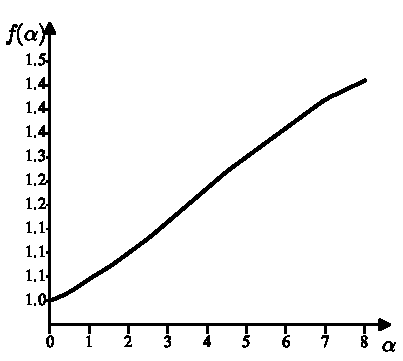
\includegraphics[width=6cm]{fig9-1.pdf}\\{\small 图 9.1\quad $f(\alpha)$曲线}
\end{minipage}
\end{center}

\section{小极化子理论}

在§1中我们已经指出，当电子与LO声子的耦合很强时，电子将被自己产生的极化场束缚，形成局域的极化子状态，其尺寸与晶格常数相近，称为小极化子.显然，对于小极化子问题不能再用连续模型处理，必须从晶格模型出发，同时考虑周期场和电子-LO声子相互作用对载流子（电子或空穴）能态的影响.小极化子在晶格中运动有两种不同方式：其一是能带传导，其二是跳跃过程（hopping processes）.在低温区，小极化子从一格点向邻近格点转移时往往不改变声子组态，在此近似之下系统具有平移对称性，可以形成小极化子的能带状态，它与紧束缚近似中电子的运动相似，不同之处在于计入了晶格振动的影响.涉及到有限温度时非刚性晶格的紧束缚近似能带问题.随着温度升高在小极化子周围的声子数增多，会导致能带传导电子的有效质量增大，从而使极化子带宽变窄.不难想象，存在一个转变温度 $T_{\mathrm t}$，当 $T>T_{\mathrm t}$ 时小极化子的能带宽度将小于它的能量不确定度（$\sim\hbar/\tau$，$\tau$ 是寿命），这时小极化子能带状态不再是系统的定态，极化子的能带图像失效，其运动将改变方式.在高温区小极化子基本上是局域粒子，它只能依靠热声子激活从一格点向另一格点作跳跃运动，与晶格缺陷的扩散运动相似，是一种无规运动并伴随着热声子的产生和消灭（声子组态变化），这种运动方式称为跳跃过程.在本节中我们将采用电子与LO声子耦合的晶格模型\textsuperscript{[13]}来讨论小极化子的能带传导和跳跃过程.

\subsection*{1. 小极化子的哈密顿量}

在三维晶格中电子与LO声子互作用系统由
\begin{equation}
  H=H_{\mathrm e}+H_{\mathrm p}+H_{\mathrm{int}}
\end{equation}
描述，其中
\begin{equation}
  H_{\mathrm e}=\mathscr{E}_{0}\sum_{l}C_{l}^{+}C_{l}
  -J\sum_{l}\sum_{\rho}C_{l+\rho}^{+}C_{l}
\end{equation}
代表电子在晶格周期场中运动的紧束缚近似哈密顿量. $C_{l}$，$C_{l}^{+}$ 是瓦尼尔表象中的电子算符，$\boldsymbol{\rho}$ 代表最近邻格点的位置矢，J为交迭积分，$\mathscr{E}_{0}$ 则代表在任一格点周围分子轨道态能量.
\begin{equation}
  H_{\mathrm p}=\sum_{q}\hbar\omega_{q}
  \biggl(a_{q}^{+}a_{q}+\frac{1}{2}\biggr)
\end{equation}
$a_{q}$、$a_{q}^{+}$ 为LO声子算符，LO声子频率 $\omega_{q}=\omega_{-q}$，具有时间反演对称性.
\begin{equation}
\begin{aligned}
  &H_{\mathrm{int}}=\sum_{q,l}M_{q}\,\mathrm{e}^{\mathrm{i}\boldsymbol{q}\cdot\boldsymbol{l}}
  \bigl(a_{q}+a_{-q}^{+}\bigr)C_{l}^{+}C_{l}\\
  &M_{q}^{*}=M_{-q}
\end{aligned}
\end{equation}
代表晶格模型的电子-LO声子互作用项.式(9.4.4)可仿照第五章§2从瓦尼尔表象导出，其主要步骤如下：

瓦尼尔表象中电子的态矢量
\begin{equation*}
  \varPsi(\boldsymbol{r})=\frac{1}{\sqrt{N}}\sum_{l}C_{l}\,
  a\bigl(\boldsymbol{r}-\boldsymbol{l}\bigr)
\end{equation*}
其中 $a\bigl(\boldsymbol{r}-\boldsymbol{l}\bigr)$ 是瓦尼尔函数.电子-声子互作用的二次量子化表示按常规写成
\begin{equation}
\begin{aligned}
  H_{\mathrm{int}}&=\int\varPsi^{+}(\boldsymbol{r})h(\boldsymbol{r})
  \varPsi(\boldsymbol{r})\,\mathrm{d}\boldsymbol{r}\\
  &=\frac{1}{N}\sum_{l,l'}C_{l}^{+}C_{l}
  \int a^{*}\bigl(\boldsymbol{r}-\boldsymbol{l}'\bigr)h(\boldsymbol{r})
  a\bigl(\boldsymbol{r}-\boldsymbol{l}\bigr)\mathrm{d}\boldsymbol{r}\\
  &\approx\frac{1}{N}\sum_{l}C_{l}^{+}C_{l}
  \int\bigl|a(\boldsymbol{r}-\boldsymbol{l})\bigr|^{2}h(\boldsymbol{r})\,
  \mathrm{d}\boldsymbol{r}
\end{aligned}
\end{equation}
上式的最后一个等号中略去了多中心积分，因为小极化子属于强耦合情况，电子主要是在 $\boldsymbol{l}$ 格点附近的局域轨道上感受到位移的作用.其中 $h(\boldsymbol{r})$ 是晶格位移对单电子作用的势能，对于复式晶格
\begin{equation}
  h(\boldsymbol{r})=-\sum_{l,s}\boldsymbol{u}_{l}(s)\cdot
  \nabla\,v_{s}\bigl(\boldsymbol{r}-\boldsymbol{l}-\boldsymbol{d}_{s}\bigr)
\end{equation}
$\boldsymbol{d}_{s}$ 代表第s原子在元胞中的位置，$v_{s}$ 为原子势，其总和构成晶格周期场
\begin{equation}
  V(\boldsymbol{r})=\sum_{l,s}v_{s}\bigl(\boldsymbol{r}-\boldsymbol{l}
  -\boldsymbol{d}_{s}\bigr)
\end{equation}
复式晶格的位移，根据第二章可写为
\begin{equation}
  \boldsymbol{u}_{l}(s)=\sum_{q,j}
  \sqrt{\frac{\hbar}{2NM_{s}\omega_{qj}}}\,
  \boldsymbol{e}_{qj}\bigl(a_{qj}+a_{-qj}^{+}\bigr)
  \mathrm{e}^{\mathrm{i}\boldsymbol{q}\cdot\boldsymbol{l}}
\end{equation}
其中 $j$ 为声子频谱的支指标.将式(9.4.8)和(9.4.6)代入式(9.4.5)，经整理得到
\begin{equation}
  H_{\mathrm{int}}=\sum_{q,l}\sum_{j}M_{qj}\,
  \mathrm{e}^{\mathrm{i}\boldsymbol{q}\cdot\boldsymbol{l}}
  \bigl(a_{qj}+a_{-qj}^{+}\bigr)C_{l}^{+}C_{l}
\end{equation}
\begin{equation}
  M_{qj}=-\mathrm{i}\sum_{s}
  \sqrt{\frac{\hbar}{2NM_{s}\omega_{qj}}}\,
  \mathrm{e}^{-\mathrm{i}\boldsymbol{q}\cdot\boldsymbol{d}_{s}}v_{s}(\boldsymbol{q})
  \bigl[\boldsymbol{e}_{q}(s)\cdot\boldsymbol{q}\bigr]
  \int\bigl|a(\boldsymbol{r})\bigr|^{2}
  \mathrm{e}^{-\mathrm{i}\boldsymbol{q}\cdot\boldsymbol{r}}\mathrm{d}\boldsymbol{r}
\end{equation}
其中 $v_{s}(\boldsymbol{q})$ 是原子势 $v_{s}(\boldsymbol{r})$ 的傅里叶变换，由关系式
$v_{s}(-\boldsymbol{q})=v_{s}^{*}(\boldsymbol{q})$、$\omega_{-qj}=\omega_{qj}$ 和
$\boldsymbol{e}_{-qj}=\boldsymbol{e}_{qj}^{*}$ 可求得
\begin{equation*}
  \boldsymbol{M}_{-\boldsymbol{q}j}=\boldsymbol{M}_{\boldsymbol{q}j}^{*}
\end{equation*}
如果只考虑LO声子与电子相互作用，则式(9.4.9)中对频谱支指标j的求和可去掉，就得到 $H_{\mathrm{int}}$ 的表示式(9.4.4)了.

\subsection*{2. 位移振子变换}

将 $H_{\mathrm e}$、$H_{\mathrm p}$ 和 $H_{\mathrm{int}}$ 代入式(9.4.1)，小极化子的哈密顿量可重新归并为下列两项之和为
\begin{equation}
  H=H_{0}+H_{1}
\end{equation}
其中
\begin{equation}
  H_{0}=\sum_{l}\biggl\{\mathscr{E}_{0}C_{l}^{+}C_{l}
  +C_{l}^{+}C_{l}\sum_{q}M_{q}\mathrm{e}^{\mathrm{i}\boldsymbol{q}\cdot\boldsymbol{l}}
  \bigl(a_{q}+a_{-q}^{+}\bigr)\biggr\}
  +\sum_{q}\hbar\omega_{q}\bigl(a_{q}^{+}a_{q}+1/2\bigr)
\end{equation}
描述l格点周围局域极化子状态，而
\begin{equation}
  H_{1}=-J\sum_{l,\rho}C_{l+\rho}^{+}C_{l}
\end{equation}
则代表小极化子在晶格中运动项.由于小极化子运动涉及窄能带中载流子迁移问题，其迁移率比较小，可将 $H_{1}$ 当微扰项处理.但是，对于 $H_{0}$ 项，其中包括电子与LO声子的强耦合作用，必须用非微扰方法求解.对于单个极化子问题，可以利用位移振子变换技巧将 $H_{0}$ 对角化，求得局域极化子的本征态.

对H作下列幺正变换：
\begin{equation}
  \overline{H}=\mathrm{e}^{-S}H\mathrm{e}^{S}
  =\overline{H}_{0}+\overline{H}_{1}
\end{equation}
其中母函数S取为
\begin{equation}
  S=\sum_{q,l}\frac{M_{q}}{\hbar\omega_{q}}\,
  \mathrm{e}^{\mathrm{i}\boldsymbol{q}\cdot\boldsymbol{l}}C_{l}^{+}C_{l}
  \bigl(a_{q}+a_{-q}^{+}\bigr)
\end{equation}
变换后的声子算符为
\begin{equation}
\left.
\begin{aligned}
  &\mathrm{e}^{-S}a_{q}\mathrm{e}^{S}=a_{q}
  -\sum_{l}\frac{M_{q}^{*}}{\hbar\omega_{q}}\,
  \mathrm{e}^{-\mathrm{i}\boldsymbol{q}\cdot\boldsymbol{l}}C_{l}^{+}C_{l}\\
  &\mathrm{e}^{-S}a_{q}^{+}\mathrm{e}^{S}=a_{q}^{+}
  -\sum_{l}\frac{M_{q}}{\hbar\omega_{q}}\,
  \mathrm{e}^{\mathrm{i}\boldsymbol{q}\cdot\boldsymbol{l}}C_{l}^{+}C_{l}
\end{aligned}\right\}
\end{equation}
相当于作了原点位移.电子算符 $C_{l}$ 与 $C_{l}^{+}$ 经变换成为
\begin{equation}
\left.
\begin{aligned}
  &\mathrm{e}^{-S}C_{l}\mathrm{e}^{S}=C_{l}X_{l}\\
  &\mathrm{e}^{-S}C_{l}^{+}\mathrm{e}^{S}=C_{l}^{+}X_{l}^{+}
\end{aligned}\right\}
\end{equation}
其中
\begin{equation}
  X_{l}=\exp\biggl\{\sum_{q}\biggl(\frac{M_{q}}{\hbar\omega_{q}}\biggr)
  \mathrm{e}^{\mathrm{i}\boldsymbol{q}\cdot\boldsymbol{l}}
  \bigl(a_{q}-a_{-q}^{+}\bigr)\biggr\}
\end{equation}
它只含声子算符.由于 $M_{-q}^{*}=M_{q}$ 以及 $\omega_{-q}=\omega_{q}$，对于同一格点有算符等式
\begin{equation}
  X_{l}^{+}X_{l}=1
\end{equation}
因此，变换对 $H_{0}$ 中对角项 $C_{l}^{+}C_{l}$ 无影响，只对 $H_{1}$ 有影响.将以上结果代入式(9.4.14)可得
\begin{equation}
  \overline{H}_{1}=-J\sum_{l}\sum_{\rho}'
  C_{l+\rho}^{+}C_{l}X_{l+\rho}^{+}X_{l}
\end{equation}
\begin{equation}
  \overline{H}_{0}=\sum_{l}\bigl(\mathscr{E}_{0}-\Delta\bigr)C_{l}^{+}C_{l}
  +\sum_{q}\hbar\omega_{q}\biggl(a_{q}^{+}a_{q}+\frac{1}{2}\biggr)
  +\sum_{l\neq l'}\sum U\bigl(\boldsymbol{l}-\boldsymbol{l}'\bigr)
  C_{l}^{+}C_{l'}^{+}C_{l'}C_{l}
\end{equation}
上式中右边最后一项代表 $\boldsymbol{l}$ 处与 $\boldsymbol{l}'$ 处两个局域极化子的有效互作用，其中
\begin{equation}
  U\bigl(\boldsymbol{l}-\boldsymbol{l}'\bigr)\equiv
  -\sum_{q}\biggl(\frac{\bigl|M_{q}\bigr|^{2}}{\hbar\omega_{q}}\biggr)
  \mathrm{e}^{\mathrm{i}\boldsymbol{q}\cdot(\boldsymbol{l}-\boldsymbol{l}')}
\end{equation}
它对于双极化子问题的研究有重要作用，在单极化子问题中这一项可以略去，于是求得单个局域极化子的对角化哈密顿量
\begin{equation}
  H_{0}\approx\sum_{l}\bigl(\mathscr{E}_{0}-\Delta\bigr)C_{l}^{+}C_{l}
  +\sum_{q}\hbar\omega_{q}\biggl(a_{q}^{+}a_{q}+\frac{1}{2}\biggr)
\end{equation}
这里
\begin{equation}
  \Delta\equiv\sum_{q}\frac{\bigl|M_{q}\bigr|^{2}}{\hbar\omega_{q}}
\end{equation}
是 $H_{\mathrm{int}}$ 对 $\mathscr{E}_{0}$ 的修正.由 $\overline{H}_{0}$ 描述的l格点局域极化子状态可写成
\begin{equation}
  |1_{l}\rangle\prod_{q}|n_{q}\rangle
  \equiv|1_{l}\rangle\,|\{n_{q}\}\rangle
\end{equation}
$\prod\limits_{q}|n_{q}\rangle$ 是极化子的声子组态，$n_{q}$ 代表 $\boldsymbol{q}$ 波矢的LO声子数.

现在讨论微扰项 $\overline{H}_{1}$ 的作用，利用式(9.4.25)和(9.4.20)，立刻求得小极化从 $\boldsymbol{l}$ 格点向 $\boldsymbol{l}+\boldsymbol{\rho}$ 格点跃迁矩阵元为
\begin{equation*}
  -J\langle f|X_{l+\rho}^{+}X_{l}|i\rangle
\end{equation*}
其中 $|i\rangle=|\{n_{q}\}\rangle$ 和 $|f\rangle=|\{n_{q}'\}\rangle$ 为跃迁前后的声子组态.由于 $X_{l+\rho}^{+}X_{l}$ 允许声子的产生和消灭，因此从态 $|i\rangle$ 向 $|f\rangle$ 跃迁时可能出现两种情况：

（i）对角跃迁：这时 $|i\rangle=|f\rangle$，跃迁前后声子组态不变，可以建立小极化子能带理论.

（ii）非对角跃迁：$|i\rangle\neq|f\rangle$，声子组态发生了改变，从 $\boldsymbol{l}$ 向 $\boldsymbol{l}+\boldsymbol{\rho}$ 跃迁伴随着声子数的变化，属于跳跃运动过程.

下面将分别介绍这两种跃迁过程.

\subsection*{3. 小极化子的能带理论}

如果只发生对角跃迁，小极化子从 $\boldsymbol{l}$ 向 $\boldsymbol{l}+\boldsymbol{\rho}$ 运动时各个 $\boldsymbol{q}$ 态的声子数均无变化，在这样的限制条件下，小极化子在晶格中运动具有平移对称性，可以应用布洛赫定理构成小极化子的能带状态
\begin{equation}
  |1_{k},\{n_{q}\}\rangle=\frac{1}{\sqrt{N}}\sum_{l}
  \mathrm{e}^{\mathrm{i}\boldsymbol{k}\cdot\boldsymbol{l}}|1_{l}\rangle
  \prod_{q}|n_{q}\rangle
\end{equation}
用上述布洛赫态对 $\overline{H}$ 求对角平均，得到 $\{n_{q}\}$ 声子组态的小极化子能带曲线
\begin{equation}
\begin{aligned}
  E_{k}(\{n_{q}\})&=\bigl\langle 1_{k},\{n_{q}\}\bigl|\overline{H}
  \bigr|1_{k},\{n_{q}\}\bigr\rangle\\
  &=\bigl(\mathscr{E}_{0}-\Delta\bigr)
  +\sum_{q}\hbar\omega_{q}\biggl(n_{q}+\frac{1}{2}\biggr)\\
  &\quad-J\sum_{\rho}\mathrm{e}^{-\mathrm{i}\boldsymbol{k}\cdot\boldsymbol{\rho}}
  \prod_{q}\bigl\langle n_{q}\bigl|\exp(\lambda_{q}^{*}a_{q}^{+}
  -\lambda_{q}a_{q})\bigr|n_{q}\bigr\rangle
\end{aligned}
\end{equation}
这里系数
\begin{equation}
  \lambda_{q}\equiv-\left(M_{q}/\hbar\omega_{q}\right)
  \mathrm{e}^{\mathrm{i}\boldsymbol{q}\cdot\boldsymbol{l}}
  \bigl(1-\mathrm{e}^{\mathrm{i}\boldsymbol{q}\cdot\boldsymbol{\rho}}\bigr)
\end{equation}
有限温度T时小极化子能带曲线应由式(9.4.27)对声子部分统计平均得到
\begin{equation}
\begin{aligned}
  E_{k}(T)&=\bigl(\mathscr{E}_{0}-\Delta\bigr)
  +\sum_{q}\hbar\omega_{q}\biggl(\langle n_{q}\rangle_{T}
  +\frac{1}{2}\biggr)\\
  &\quad-J\sum_{\rho}\mathrm{e}^{\mathrm{i}\boldsymbol{k}\cdot\boldsymbol{\rho}}
  \prod_{q}\bigl\langle\exp(\lambda_{q}^{*}a_{q}^{+}-\lambda_{q}a_{q})
  \bigr\rangle_{T}
\end{aligned}
\end{equation}
其中
\begin{equation}
\begin{aligned}
  \langle n_{q}\rangle_{T}
  &=\bigl(1-\mathrm{e}^{-\beta\hbar\omega_{q}}\bigr)
  \sum_{n_{q}=0}^{\infty}n_{q}\bigl(\mathrm{e}^{-\beta\hbar\omega_{q}}\bigr)^{n_{q}}\\
  &=\bigl(\mathrm{e}^{\beta\hbar\omega_{q}}-1\bigr)^{-1}
  \quad\bigl[\beta=\left(k_{\mathrm B}T\right)^{-1}\bigr]\\
  \bigl\langle\exp\bigl(\lambda_{q}^{*}a_{q}^{+}-\lambda_{q}a_{q}\bigr)
  \bigr\rangle_{T}
  &=\mathrm{e}^{-\frac{1}{2}|\lambda_{q}|^{2}}
  \bigl\langle\mathrm{e}^{\lambda_{q}^{*}a_{q}^{+}}
  \mathrm{e}^{-\lambda_{q}a_{q}}\bigr\rangle_{T}\\
  &=\mathrm{e}^{-\frac{1}{2}|\lambda_{q}|^{2}}
  \bigl(1-\mathrm{e}^{-\beta\hbar\omega_{q}}\bigr)\times
\end{aligned}
\end{equation}
\begin{equation}
  \sum_{n,q}^{\infty}\bigl\langle n_{q}\bigl|
  \mathrm{e}^{\lambda_{q}^{*}a_{q}^{+}}\mathrm{e}^{-\lambda_{q}a_{q}}
  \bigr|n_{q}\bigr\rangle\mathrm{e}^{-\beta n_{q}\hbar\omega_{q}}
\end{equation}
这里应用了算符等式
$\mathrm{e}^{\hat{A}+\hat{B}}
=\mathrm{e}^{-\frac{1}{2}[\hat{A},\hat{B}]}\mathrm{e}^{\hat{A}}\mathrm{e}^{\hat{B}}$.利用声子算符于本征态，容易求得下列关系：
\begin{equation}
\begin{aligned}
  &\mathrm{e}^{-\lambda a}|n\rangle=\sum_{p=0}^{\infty}
  \frac{(-\lambda)^{p}}{p!}\,a^{p}|n\rangle
  =\sum_{p=0}^{\infty}\frac{(-\lambda)^{p}}{p!}
  \biggl[\frac{n!}{(n-p)!}\biggr]^{1/2}|n-p\rangle\\
  &\langle n|\mathrm{e}^{\lambda^{*}a^{+}}
  =\sum_{m=0}^{\infty}\frac{(\lambda^{*})^{m}}{m!}
  \biggl[\frac{n!}{(n-m)!}\biggr]^{1/2}\langle n-m|\\
  &\langle n-m|n-p\rangle=\delta_{pm}
\end{aligned}
\end{equation}
由此算出
\begin{equation}
\begin{aligned}
  \bigl\langle n\bigl|\mathrm{e}^{\lambda^{*}a^{+}}
  \mathrm{e}^{-\lambda a}\bigr|n\bigr\rangle
  &=\sum_{m=0}^{n}\frac{(-|\lambda|^{2})^{m}}{(m!)^{2}}\,
  \frac{n!}{(n-m)!}\\
  &=\mathrm{L}_{n}\bigl(|\lambda|^{2}\bigr)
\end{aligned}
\end{equation}
$\mathrm{L}_{n}$ 为拉盖尔（Laguerre）多项式.再利用拉盖尔多项式的生成函数关系
\begin{equation}
  \left(1-Z\right)^{-1}
  \mathrm{e}^{\left[|\lambda|^{2}Z/(Z-1)\right]}
  =\sum_{n=0}^{\infty}\mathrm{L}_{n}\bigl(|\lambda|^{2}\bigr)Z^{n}
\end{equation}
并令
\begin{equation*}
  Z\equiv\mathrm{e}^{-\beta\hbar\omega_{q}}
\end{equation*}
所以
\begin{equation}
  \frac{Z}{Z-1}=\langle n_{q}\rangle_{T}
\end{equation}
可得
\begin{equation}
\begin{aligned}
  \mathrm{e}^{-S_{T}}&\equiv\prod_{q}
  \bigl\langle\exp(\lambda_{q}^{*}a_{q}^{+}-\lambda_{q}a_{q})
  \bigr\rangle_{T}\\
  &=\exp\biggl[-\sum_{q}|\lambda_{q}|^{2}
  \biggl(\langle n_{q}\rangle_{T}+\frac{1}{2}\biggr)\biggr]
\end{aligned}
\end{equation}
因此小极化子能带为
\begin{equation}
  E_{k}(T)=E_{0}(T)-J\sum_{\rho}\mathrm{e}^{-S_{T}}
  \mathrm{e}^{-\mathrm{i}\boldsymbol{k}\cdot\boldsymbol{\rho}}
\end{equation}
其中
\begin{equation}
  E_{0}(T)\equiv\bigl(\mathscr{E}_{0}-\Delta\bigr)
  +\sum_{q}\hbar\omega_{q}\biggl(\langle n_{q}\rangle_{T}
  +\frac{1}{2}\biggr)
\end{equation}
\begin{equation}
\begin{aligned}
  S_{T}&=\sum_{q}|\lambda_{q}|^{2}
  \biggl(\langle n_{q}\rangle_{T}+\frac{1}{2}\biggr)\\
  &=\sum_{q}\biggl\{\frac{|M_{q}|^{2}}{\left(\hbar\omega_{q}\right)^{2}}
  \bigl|1-\mathrm{e}^{-\mathrm{i}\boldsymbol{q}\cdot\boldsymbol{\rho}}\bigr|^{2}
  \biggl(\langle n_{q}\rangle_{T}+\frac{1}{2}\biggr)\biggr\}\\
  &=\sum_{q}\biggl\{2\,\frac{|M_{q}|^{2}}{\left(\hbar\omega_{q}\right)^{2}}
  \sin^{2}\biggl(\frac{\boldsymbol{q}\cdot\boldsymbol{\rho}}{2}\biggr)
  \coth\biggl(\frac{\hbar\omega_{q}}{2k_{\mathrm B}T}\biggr)\biggr\}
\end{aligned}
\end{equation}
这里对 $\boldsymbol{q}$ 求和后 $S_{T}$ 与 $\boldsymbol{\rho}$ 的取向无关，可将 $\mathrm{e}^{-S_{T}}$ 因子从求和号中抽出，最后得到有限温度能带
\begin{equation}
  E_{k}(T)=E_{0}(T)-J\mathrm{e}^{-S_{T}}
  \sum_{\rho}\mathrm{e}^{-\mathrm{i}\boldsymbol{k}\cdot\boldsymbol{\rho}}
\end{equation}
与第八章§10中刚性晶格的紧束缚近似能带相比较，求得小极化子的能带半宽为
\begin{equation}
  ZJ\exp\left(-S_{T}\right)
\end{equation}
由于 $\exp\left(-S_{T}\right)$ 随温度升高减小，因此小极化子的能带宽度随温度升高变窄.这是小极化子能带不同于刚性晶格电子能带的特征.应当注意到，即使在绝对零度时小极化子的能带半宽仍比 $ZJ$ 小，它等于
\begin{equation*}
  ZJ\exp\left(-S_{0}\right)
\end{equation*}
其中
\begin{equation*}
  S_{0}=\frac{1}{2}\sum_{q}
  \frac{\bigl|M_{q}\bigr|^{2}}{\left(\hbar\omega_{q}\right)^{2}}
  \bigl|1-\mathrm{e}^{\mathrm{i}\boldsymbol{q}\cdot\boldsymbol{\rho}}\bigr|^{2}
\end{equation*}
零温带宽变窄效应是由于电子与LO虚声子互作用（通过零点振动）引起极化子有效质量增大所导致.

为了得到小极化子能带理论的成立条件，还必须估计非对角跃迁的作用.既然，对角跃迁给出小极化子的能带状态 $\left(\boldsymbol{k},\{n_{q}\}\right)$，那么计入非对角跃迁必将引起极化子从 $\left(\boldsymbol{k},\{n_{q}\}\right)$ 态向其它态 $\left(\boldsymbol{k}',\{n_{q}'\}\right)$ 的散射.小极化子在某一能带态的平均寿命 $\tau$ 等于总散射概率的倒数，而 $\left(\hbar/\tau\right)$ 则代表小极化处于带状态的能量不确定度.只有当 $\left(\hbar/\tau\right)$ 远远小于能带半宽度时，才能认为小极化子的能带解是系统的稳定状态.反之，小极化子的能带图像就失去意义了，这时必须计算非对角跃迁概率.

\subsection*{4. 小极化子的跳跃运动}

现在讨论小极化子从 $\boldsymbol{l}$ 向 $\boldsymbol{l}+\boldsymbol{\rho}$ 格点运动的非对角跃迁过程，即声子激活跳跃机制.根据含时微扰理论\textsuperscript{[14]}，跃迁概率（定义为每秒跳跃次数）w 与跃迁矩阵元
$\langle f|X_{l+\rho}^{+}X_{l}|i\rangle$ 关系为
\begin{equation}
  w=\frac{1}{\hbar^{2}}\int_{-\infty}^{\infty}\mathrm{d}t\,W(t)
\end{equation}
其中
\begin{equation}
\begin{aligned}
  W(t)&\equiv J^{2}\sum_{f\neq i}
  \bigl\langle i\bigl|X_{l}^{+}(t)X_{l+\rho}(t)\bigr|f\bigr\rangle
  \bigl\langle f\bigl|X_{l+\rho}^{+}X_{l}\bigr|i\bigr\rangle\\
  &=J^{2}\bigl\{\bigl\langle i\bigl|X_{l}^{+}(t)X_{l+\rho}(t)
  X_{l+\rho}^{+}X_{l}\bigr|i\bigr\rangle
  -\bigl|\bigl\langle i\bigl|X_{l+\rho}^{+}X_{l}\bigr|i\bigr\rangle\bigr|^{2}\bigr\}
\end{aligned}
\end{equation}
\begin{equation}
  X_{l}(t)=\mathrm{e}^{\mathrm{i}\overline{H}_{0}t/\hbar}X_{l}
  \mathrm{e}^{-\mathrm{i}\overline{H}_{0}t/\hbar}
\end{equation}
对角跃迁矩阵元为
\begin{equation}
  \bigl\langle i\bigl|X_{l+\rho}^{+}X_{l}\bigr|i\bigr\rangle
  =\prod_{q}\bigl\langle n_{q}\bigl|\exp(\lambda_{q}^{*}a_{q}^{+}
  -\lambda_{q}a_{q})\bigr|n_{q}\bigr\rangle
\end{equation}
其统计平均值为 $\exp\left(-S_{T}\right)$，并在热力学极限近似用 $\exp\left(-2S_{T}\right)$ 表示
$\bigl|\langle i|X_{l+\rho}^{+}X_{l}|i\rangle\bigr|^{2}$，由式(9.4.18)和(9.4.28)求得W中的时间关联函数
\begin{equation}
\begin{aligned}
  &\bigl\langle i\bigl|X_{l}^{+}(t)X_{l+\rho}(t)X_{l+\rho}^{+}X_{l}
  \bigr|i\bigr\rangle\\
  &\quad=\bigl\langle i\bigl|\exp\biggl\{\sum_{q}\biggl[
  \biggl(\lambda_{q}a_{q}+\frac{1}{2}\bigl|\lambda_{q}\bigr|^{2}\biggr)
  \bigl(\mathrm{e}^{-\mathrm{i}\omega_{q}t}-1\bigr)\\
  &\qquad-\biggl(\lambda_{q}^{*}a_{q}^{+}
  +\frac{1}{2}\bigl|\lambda_{q}\bigr|^{2}\biggr)
  \bigl(\mathrm{e}^{\mathrm{i}\omega_{q}t}-1\bigr)\biggr]\biggr\}
  \biggr|i\bigr\rangle\\
  &\quad=\exp\biggl[-\frac{1}{2}\sum_{q}B_{q}\biggr]\prod_{q}
  \bigl\langle n_{q}\bigl|\exp\bigl(A_{q}^{*}a_{q}^{+}-A_{q}a_{q}\bigr)
  \bigr|n_{q}\bigr\rangle
\end{aligned}
\end{equation}
其中 $\lambda_{q}$ 由式(9.4.28)定义，而
\begin{equation*}
\begin{aligned}
  &A_{q}\equiv-\lambda_{q}\bigl(\mathrm{e}^{-\mathrm{i}\omega_{q}t}-1\bigr)\\
  &B_{q}\equiv|\lambda_{q}|^{2}
  \bigl[\bigl(\mathrm{e}^{\mathrm{i}\omega_{q}t}-1\bigr)
  -\bigl(\mathrm{e}^{-\mathrm{i}\omega_{q}t}-1\bigr)\bigr]
\end{aligned}
\end{equation*}
式(9.4.46)中含声子算符 $a_{q}$ 与 $a_{q}^{+}$ 部分的统计平均为
\begin{equation*}
  \prod_{q}\bigl(1-\mathrm{e}^{-\beta\hbar\omega_{q}}\bigr)
  \sum_{n_{q}=0}^{\infty}\bigl(\mathrm{e}^{-\beta\hbar\omega_{q}}\bigr)^{n_{q}}
  \bigl\langle n_{q}\bigl|\mathrm{e}^{A_{q}^{*}a_{q}^{+}-A_{q}a_{q}}
  \bigr|n_{q}\bigr\rangle
\end{equation*}
作类似于上节的计算，利用式(9.4.36)求得
\begin{equation}
  \bigl\langle X_{l}^{+}(t)X_{l+\rho}(t)X_{l+\rho}^{+}X_{l}
  \bigr\rangle_{T}
  =\exp\{-2S_{T}+\varphi(t)\}
\end{equation}
其中 $S_{T}$ 由式(9.4.39)决定，而
\begin{equation}
\begin{aligned}
  \varphi(t)&=\sum_{q}|\lambda_{q}|^{2}
  \bigl\{\bigl(\langle n_{q}\rangle_{T}+1\bigr)
  \mathrm{e}^{-\mathrm{i}\omega_{q}t}
  +\langle n_{q}\rangle_{T}\mathrm{e}^{\mathrm{i}\omega_{q}t}\bigr\}\\
  &=2\sum_{q}|\lambda_{q}|^{2}
  \bigl[\langle n_{q}\rangle_{T}\bigl(\langle n_{q}\rangle_{T}+1\bigr)
  \bigr]^{1/2}
  \cos\biggl[\omega_{q}\biggl(t+\frac{\mathrm{i}\beta\hbar}{2}\biggr)\biggr]
\end{aligned}
\end{equation}
其中利用了下列关系式：
\begin{equation*}
  \sqrt{\frac{\langle n_{q}\rangle_{T}+1}{\langle n_{q}\rangle_{T}}}
  =\mathrm{e}^{\frac{1}{2}\beta\hbar\omega_{q}}\,,\quad
  \sqrt{\frac{\langle n_{q}\rangle_{T}}{\langle n_{q}\rangle_{T}+1}}
  =\mathrm{e}^{-\frac{1}{2}\beta\hbar\omega_{q}}
\end{equation*}
将式(9.4.48)代入式(9.4.43)和(9.4.42)，可得w的统计平均值为
\begin{equation}
  w_{T}=\frac{J^{2}}{\hbar^{2}}\mathrm{e}^{-2S_{T}}
  \int_{-\infty}^{\infty}\mathrm{d}t\,
  \bigl(\mathrm{e}^{\varphi(t)}-1\bigr)
\end{equation}
在三维情况下被积函数收敛很快，可将 $\varphi(t)$ 延拓到 t 的复平面z上成为
\begin{equation}
  \varphi(z)=2\sum_{q}|\lambda_{q}|^{2}
  \bigl[\langle n_{q}\rangle_{T}
  \bigl(\langle n_{q}\rangle_{T}+1\bigr)\bigr]^{1/2}
  \cos\omega_{q}z
\end{equation}
在 $z=0$ 附近展开 $\varphi(z)$，得
\begin{equation*}
  \varphi(z)\approx\varphi(0)-\gamma z^{2}+\cdots,
\end{equation*}
\begin{equation}
  \varphi(0)=2\sum_{q}|\lambda_{q}|^{2}
  \bigl[\langle n_{q}\rangle_{T}
  \bigl(\langle n_{q}\rangle_{T}+1\bigr)\bigr]^{1/2}
\end{equation}
\begin{equation}
  \gamma=\sum_{q}\omega_{q}^{2}|\lambda_{q}|^{2}
  \bigl[\langle n_{q}\rangle_{T}
  \bigl(\langle n_{q}\rangle_{T}+1\bigr)\bigr]^{1/2}
\end{equation}
代入式(9.4.49)作回路积分\textsuperscript{[13]}
\begin{equation}
\begin{aligned}
  w_{T}&=\frac{J^{2}}{\hbar^{2}}\mathrm{e}^{-2S_{T}}
  \int\mathrm{d}z\,\bigl(\mathrm{e}^{\varphi(z)}-1\bigr)\\
  &\approx\frac{J^{2}}{\hbar^{2}}
  \biggl\{\int_{-\infty}^{\infty}\mathrm{d}z\,\mathrm{e}^{-\gamma z^{2}}
  \biggr\}\exp\bigl[-2S_{T}+\varphi(0)\bigr]\\
  &\approx\frac{J^{2}}{\hbar^{2}}
  \biggl(\frac{\pi}{\gamma}\biggr)^{\frac{1}{2}}
  \exp\bigl[-2S_{T}+\varphi(0)\bigr]
\end{aligned}
\end{equation}
再将 $\langle n_{q}\rangle_{T}$ 和 $\lambda_{q}$ 代入 $S_{T}$ 及 $\varphi(0)$ 中，在高温近似下求出
\begin{equation}
\begin{aligned}
  2S_{T}-\varphi(0)&=\sum_{q}\frac{|M_{q}|^{2}}
  {\left(\hbar\omega_{q}\right)^{2}}
  \bigl|1-\mathrm{e}^{\mathrm{i}\boldsymbol{q}\cdot\boldsymbol{\rho}}\bigr|^{2}
  \bigl\{\bigl(2\langle n_{q}\rangle_{T}+1\bigr)\\
  &\quad-2\bigl[\langle n_{q}\rangle_{T}
  \bigl(\langle n_{q}\rangle_{T}+1\bigr)\bigr]^{1/2}\bigr\}\\
  &\approx\sum_{q}\frac{|M_{q}|^{2}}{\left(\hbar\omega_{q}\right)^{2}}
  \bigl|1-\mathrm{e}^{\mathrm{i}\boldsymbol{q}\cdot\boldsymbol{\rho}}\bigr|^{2}
  \frac{\hbar\omega_{q}}{4k_{\mathrm B}T}
\end{aligned}
\end{equation}
定义一个能量
\begin{equation}
  E_{\mathrm a}\equiv\frac{1}{4}\sum_{q}
  \biggl(\frac{|M_{q}|}{\hbar\omega_{q}}\biggr)^{2}
  \bigl|1-\mathrm{e}^{\mathrm{i}\boldsymbol{q}\cdot\boldsymbol{\rho}}\bigr|^{2}
  \hbar\omega_{q}
\end{equation}
在高温近似下由式(9.4.52)求得
\begin{equation}
  \gamma\approx\frac{4E_{\mathrm a}k_{\mathrm B}T}{\hbar^{2}}
\end{equation}
最后得到小极化子跳跃概率的高温近似式
\begin{equation}
  w_{T}=\biggl(\frac{J}{\hbar}\biggr)^{2}
  \biggl(\frac{\pi\hbar^{2}}{4E_{\mathrm a}k_{\mathrm B}T}\biggr)^{\frac{1}{2}}
  \exp\biggl(-\frac{E_{\mathrm a}}{k_{\mathrm B}T}\biggr)
\end{equation}
它随温度升高而增大，说明小极化子靠声子热激活在晶格中作无规运动，$E_{\mathrm a}$ 可理解为跳跃运动的激活能.对于简立方晶格小极化子的扩散系数
\begin{equation}
  D=a^{2}w_{T}=\biggl(\frac{Ja}{\hbar}\biggr)^{2}
  \sqrt{\frac{\pi\hbar^{2}}{4E_{\mathrm a}k_{\mathrm B}T}}\,
  \exp\biggl(-\frac{E_{\mathrm a}}{k_{\mathrm B}T}\biggr)
\end{equation}
这里a为晶格常数.小极化子的跳跃迁移率可根据爱因斯坦关系决定
\begin{equation}
  \mu=\frac{eD}{k_{\mathrm B}T}
  =\frac{ea^{2}}{k_{\mathrm B}T}\,w_{T}
  \sim\exp\biggl(-\frac{E_{\mathrm a}}{k_{\mathrm B}T}\biggr)
\end{equation}
迁移率随温度升高而增大与晶格缺陷运动完全相似，因此人们常称小极化子状态称为晶体的一种“本征缺陷”.

\subsection*{5. 两种导电机制的转变温度$T_{\mathrm t}$}

实际上小极化子在某能带态上的寿命 $\tau$ 就是非对角跃迁概率 $w_{T}$ 的倒数.由于每个格点有z个近邻，因此 $z\hbar w_{T}$ 确定小极化子带状态的能量不确定度.当能带半宽满足条件
\begin{equation}
  J\exp\left(-2S_{T}\right)\gg\hbar w_{T}
\end{equation}
时，非对角跃迁可忽略，小极化子能带理论成立.由于 $T\to0$ K时 $w_{T}\to0$，因此低温区小极化子按能带传导方式在晶格中运动，其导电率随温度升高而降低.反过来，当T升高 $w_{T}$ 增大而 $\mathrm{e}^{-2S_{T}}$ 减小以致满足下列条件时，
\begin{equation}
  \hbar w_{T}\gg J\exp\left(-2S_{T}\right)
\end{equation}
非对角跃迁起主要作用，这时小极化子在晶格中作无规跳跃运动，其导电率随T升高增大.因此划分小极化子导电机制的转变温度应由下列等式决定：
\begin{equation*}
  \hbar w_{T_{\mathrm t}}=J\exp\left(-2S_{T_{\mathrm t}}\right)
\end{equation*}
由于 $T_{\mathrm t}$ 在中间温区，$w_{T}$ 的高温近似结果［式(9.4.57)］不能应用.文献[15]的详细计算表明，当 $\hbar\omega_{\mathrm D}/J$ 在1到100之间时，$T_{\mathrm t}$ 在 $0.4\theta_{\mathrm D}$ 到 $0.55\theta_{\mathrm D}$ 之间.这里 $\theta_{\mathrm D}$ 和 $\omega_{\mathrm D}$ 分别为德拜温度和频率.实验上也观测到了这种转变，例如 TiO$_{2}$ 的 $T_{\mathrm t}$ 大致为300℃\textsuperscript{[16]}.

现已证实，在新发现的混合价锰氧化物
$\mathrm{Re}_{1-x}\mathrm{A}_{x}\mathrm{MnO}_{3}$
（Re：La，Nd；A：Ca，Sr）组成的庞磁电阻（colossal magnetoresistance，CMR）系统中，小极化子的高温跳跃传导\textsuperscript{[17]}和低温能带传导\textsuperscript{[18]}均起重要作用.

\section{一维极化子理论}

近年来由于低维系统非线性元激发的研究进展，重新引起人们对一维极化子理论的兴趣.例如，在聚乙炔链中不仅发现了扭形孤子解，成功地预言了“分数电荷”等特殊自旋-电荷关系\textsuperscript{[19]}，而且还找到了非线性的孤波型极化子解，并成功地说明了聚乙炔中的晶格弛豫现象\textsuperscript{[20]}.这类极化子解实质上是准一维聚乙炔链中电子与LO声子相互作用所形成的自陷态，它和一维分子晶体中的局域极化子状态有密切的关系\textsuperscript{[21,22]}.因此有必要对一维极化子的分子晶体模型\textsuperscript{[15]}作简单介绍.

设系统中包含一个过剩电子和由N个双原子分子组成的线性链.每个分子对电子作用的势能设为 $U\bigl(x-R_{n},u_{n}\bigr)$，其中 $R_{n}=na$ 代为第n个分子的位置，$u_{n}$ 是第n个分子中原子间相对振动的位移，这就是分子晶体模型.根据这个模型一维极化子的哈密顿量可写成
\begin{equation}
  H=H_{\mathrm e}+H_{\mathrm p}+H_{\mathrm{int}}
\end{equation}
其中
\begin{equation}
  H_{\mathrm e}+H_{\mathrm{int}}
  =-\frac{\hbar^{2}}{2m}\frac{\mathrm{d}^{2}}{\mathrm{d}x^{2}}
  +\sum_{n=1}^{N}U\bigl(x-R_{n},u_{n}\bigr)
\end{equation}
\begin{equation}
  H_{\mathrm p}=\sum_{n=1}^{N}\biggl(
  -\frac{\hbar^{2}}{2M}\frac{\partial^{2}}{\partial u_{n}^{2}}
  +\frac{1}{2}M\omega_{0}^{2}u_{n}^{2}
  +\frac{1}{2}M\omega_{1}^{2}u_{n}u_{n+1}\biggr)
\end{equation}
M代表相对分子质心运动的折合质量，$\omega_{0}^{2}$ 与 $\omega_{1}^{2}$ 则相当于第二章中动力矩阵的“对角”与“非对角”元素，在这里只计及了分子间近邻互作用.从物理上讲，$\omega_{0}$ 代表爱因斯坦频率，$\omega_{1}^{2}u_{n}u_{n+1}$ 项则给出LO晶格振动频率的色散部分.

哈密顿量H的波函数假定为下列线性组合
\begin{equation}
  \varPsi=\sum_{n}a_{n}\bigl(u_{1},\cdots,u_{N}\bigr)
  \phi_{n}\bigl(x,u_{n}\bigr)
\end{equation}
其中 $\phi_{n}$ 为局域化的分子轨道，它满足方程
\begin{equation}
  \biggl\{-\frac{\hbar^{2}}{2m}\frac{\mathrm{d}^{2}}{\mathrm{d}x^{2}}
  +U\bigl(x-R_{n},u_{n}\bigr)\biggr\}
  \phi_{n}\bigl(x-R_{n},u_{n}\bigr)
  =E\bigl(u_{n}\bigr)\phi_{n}\bigl(x-R_{n},u_{n}\bigr)
\end{equation}
由于各分子结构相同，因此分子轨道的本征值E只与分子振动的位移量 $u_{n}$ 有关.在线性近似范围内可将E按 $u_{n}$ 展开写为
\begin{equation*}
  E\bigl(u_{n}\bigr)=-Au_{n}+\mathrm{const.}
\end{equation*}
其中 $-Au_{n}$ 实际上代表电子与晶格振动的相互作用，因为几乎所有的电子-声子互作用都是在类似的线性展开下导出的.适当选取能量的零点，可令上式中常量项为零，于是
\begin{equation}
  E\bigl(u_{n}\bigr)=-Au_{n}
\end{equation}
式(9.5.4)中 $a_{n}\bigl(u_{1},\cdots,u_{N}\bigr)$ 是电子在n格点周围分子轨道上的概率振幅，与紧束缚近似法中的展开系数相似，不同之处在于 $a_{n}$ 随晶格振动的位形 $\left(u_{1},\cdots,u_{N}\right)$ 变化，因为现在所处理的不是刚性晶格.此外 $a_{n}$ 还是时间t的函数，下标n是代表电子状态的量子数，在这里就是格点的位标.

利用与紧束缚近似相类似的作法，可以从薛定谔方程 $\mathrm{i}\hbar\dot{\varPsi}=H\varPsi$ 导出 $a_{n}$ 的运动方程
\begin{equation}
\begin{aligned}
  \mathrm{i}\hbar\frac{\partial}{\partial t}
  a_{n}\bigl(u_{1},\cdots,u_{N}\bigr)
  &=\bigl(H_{\mathrm p}-Au_{n}\bigr)
  a_{n}\bigl(u_{1},\cdots,u_{N}\bigr)\\
  &\quad+\sum_{(\pm)}J\bigl(u_{n},u_{n\pm1}\bigr)
  a_{n\pm1}\bigl(u_{1},\cdots,u_{N}\bigr)
\end{aligned}
\end{equation}
其中
\begin{equation}
  J\bigl(u_{n},u_{m}\bigr)=\int\phi^{*}
  \bigl(\boldsymbol{x}-\boldsymbol{R}_{n},u_{n}\bigr)
  U\bigl(\boldsymbol{x}-\boldsymbol{R}_{n},u_{n}\bigr)
  \phi\bigl(\boldsymbol{x}-\boldsymbol{R}_{m},u_{m}\bigr)
  \mathrm{d}\boldsymbol{x}
\end{equation}
是双中心交迭积分.在推导过程中略去了三中心积分，只保留最近邻的双中心交迭积分.此外，还略去了 $\phi$ 对 $u_{n}$ 的导数项，文献[21]中证明了这一项作用不大，略去它相当于作绝热近似.如再略去J对u的依赖关系设 $J\bigl(u_{n},u_{n\pm1}\bigr)=-J$，并采用单频近似取 $\omega_{1}=0$，相当于用爱因斯坦模型描述LO声子，则式(9.5.7)可改写成
\begin{equation}
\begin{aligned}
  \mathrm{i}\frac{\partial}{\partial t}
  a_{n}\bigl(u_{1},\cdots,u_{N}\bigr)
  &=\sum_{m}\biggl(-\frac{\hbar^{2}}{2M}
  \frac{\partial^{2}}{\partial u_{m}^{2}}
  +\frac{1}{2}M\omega_{0}^{2}u_{m}^{2}\biggr)
  a_{n}\bigl(u_{1},\cdots,u_{N}\bigr)\\
  &\quad-J\bigl(a_{n+1}+a_{n-1}\bigr)
  -Au_{n}a_{n}\bigl(u_{1},\cdots,u_{N}\bigr)
\end{aligned}
\end{equation}
上式对任意位形 $\left(\boldsymbol{u}_{1},\cdots,\boldsymbol{u}_{N}\right)$ 求解比较困难.在强耦合情况下，电子引起晶格畸变，产生一个吸引势作用于电子本身，使电子陷落在势阱中形成自陷态，而自陷态的出现又使晶格畸变得以保持.因此，起主要作用的是晶格的静态位移，这时晶格振动的动能项对 $a_{n}$ 的影响不大，可以忽略不计.这相当于对 $a_{n}\bigl(u_{1},\cdots,u_{N}\bigr)$ 作绝热近似，并设 $a_{n}$ 有定态解，其能量本征值为 $E\bigl(u_{1},\cdots,u_{N}\bigr)$.这时式(9.5.9)简化为下列本征方程：
\begin{equation}
  \biggl\{\frac{1}{2}\sum_{m}M\omega_{0}^{2}u_{m}^{2}-Au_{n}\biggr\}a_{n}
  -J\bigl(a_{n+1}+a_{n-1}\bigr)
  =E\bigl(u_{1},\cdots,u_{N}\bigr)a_{n}
\end{equation}
将上式对 $a_{n}$ 求内积，并利用归一化条件
\begin{equation}
  1=\int|\varPsi|^{2}\mathrm{d}x=\sum_{n}|a_{n}|^{2}
\end{equation}
可求出 $E\bigl(u_{1},\cdots,u_{N}\bigr)$.系统的基态可以从 $E\bigl(u_{1},\cdots,u_{N}\bigr)$ 对 $u_{m}$ 的变分极值决定，不难算得能量极小时振动位移
$\bigl(u_{1}^{(0)},\cdots,u_{N}^{(0)}\bigr)$ 满足
\begin{equation}
  u_{m}^{(0)}=A\bigl|a_{m}^{(0)}\bigr|^{2}/M\omega_{0}^{2}
  \quad\left(m=1,2,\cdots,N\right)
\end{equation}
其中 $a_{m}^{(0)}$ 代表 $u_{m}=u_{m}^{(0)}$ 时式(9.5.10)的解.将式(9.5.12)代入式(9.5.10)，求得 $a_{n}^{(0)}$ 的方程为
\begin{equation}
  \biggl\{\frac{A^{2}}{M\omega_{0}^{2}}
  \bigl|a_{n}^{(0)}\bigr|^{2}-\mathscr{E}\biggr\}a_{n}^{(0)}
  +J\bigl(a_{n+1}^{(0)}+a_{n-1}^{(0)}-2a_{n}^{(0)}\bigr)=0
\end{equation}
其中
\begin{equation}
  \mathscr{E}\equiv\left(1/2\right)\sum_{m}M\omega_{0}^{2}
  u_{m}^{(0)2}
  -E\bigl(u_{1}^{(0)},\cdots,u_{N}^{(0)}\bigr)-2J
\end{equation}
当 $a_{n}^{(0)}$ 是n的缓变函数时，可作下列连续化近似：
\begin{equation}
  a_{n+1}^{(0)}+a_{n-1}^{(0)}-2a_{n}^{(0)}
  \approx\frac{\partial^{2}a_{n}^{(0)}}{\partial n^{2}}
\end{equation}
再定义参数
\begin{equation}
  \gamma\equiv A^{2}/4M\omega_{0}^{2}J
\end{equation}
可将 $a_{n}^{(0)}$ 的方程式(9.5.13)写成下列非线性定态薛定谔方程：
\begin{equation}
  \frac{\mathrm{d}^{2}a_{n}^{(0)}}{\mathrm{d}n^{2}}
  +4\gamma\bigl|a_{n}^{(0)}\bigr|^{2}a_{n}^{(0)}
  =\biggl(\frac{\mathscr{E}}{J}\biggr)a_{n}^{(0)}
\end{equation}
考虑方程在 $n\rightarrow\pm\infty$ 时 $a_{n}^{(0)}$ 及其导数趋向零的解，它代表极化子局域状态.这个解很容易直接求出，只要对式(9.5.17)乘以 $2\left(\mathrm{d}a_{n}/\mathrm{d}n\right)$，立刻可将上式变换为全微分，并求得其严格解为
\begin{equation}
  a_{n}^{(0)}=\sqrt{\frac{\mathscr{E}}{2\gamma J}}\,
  \mathrm{sech}\sqrt{\frac{\mathscr{E}}{J}}\,
  \left(n-n_{0}\right)
\end{equation}
其中 $n_{0}$ 是积分常数. $\mathscr{E}$ 可由归一化条件
$\sum\limits_{n}\bigl|a_{n}^{(0)}\bigr|^{2}=1$ 定出
\begin{equation}
  \mathscr{E}=J\gamma^{2}
\end{equation}
代入式(9.5.14)求得
\begin{equation}
  E\bigl(u_{1}^{(0)},\cdots,u_{N}^{(0)}\bigr)
  =-\left(1/3\right)J\gamma^{2}-2J
\end{equation}
由于2J为刚性晶格的紧束缚近似能带半宽.因此上式右边第二项-2J为能带底部电子的能量，这是周期场所造成的，而第一项则代表形成局域极化子状态时所降低的能量，因此极化子的束缚能
\begin{equation}
  E_{\mathrm p}=\frac{1}{3}J\gamma^{2}
  =\frac{1}{48J}\biggl(\frac{A^{2}}{M\omega_{0}^{2}}\biggr)^{2}
\end{equation}
局域极化子状态（即自陷态）中的晶格位移由式(9.5.18)和(9.5.12)决定：
\begin{equation}
  u_{n}^{(0)}=\frac{A}{2M\omega_{0}^{2}}\gamma\,
  \mathrm{sech}^{2}\bigl[\gamma\left(n-n_{0}\right)\bigr]
\end{equation}
相应的电子自陷势阱则为
\begin{equation}
\begin{aligned}
  V\bigl(u_{n}^{(0)}\bigr)&=E\bigl(u_{n}^{(0)}\bigr)=-Au_{n}^{(0)}\\
  &=-\frac{A^{2}}{2M\omega_{0}^{2}}\gamma\,
  \mathrm{sech}^{2}\bigl[\gamma\left(n-n_{0}\right)\bigr]
\end{aligned}
\end{equation}
根据式(9.5.18)和(9.5.19)可定出局域极化子的概率振幅：
\begin{equation}
  a_{n}^{(0)}=\sqrt{\frac{\gamma}{2}}\,
  \mathrm{sech}\bigl[\gamma\left(n-n_{0}\right)\bigr]
\end{equation}
若定义
\begin{equation}
  L_{\mathrm p}\equiv\frac{a}{\gamma}
  =\biggl(\frac{4M\omega_{0}^{2}J}{A^{2}}\biggr)a
\end{equation}
可将 $a_{n}^{(0)}$ 用 $L_{\mathrm p}$ 表示为
\begin{equation}
  a_{n}^{(0)}=\sqrt{\frac{a}{2L_{\mathrm p}}}\,
  \mathrm{sech}\biggl[\frac{\left(n-n_{0}\right)a}{L_{\mathrm p}}\biggr]
\end{equation}
其中 $\boldsymbol{a}$ 为晶格常数.显而易见，上式描述一个峰值在 $n_{0}a$ 处的钟形峰，其峰宽 $L_{\mathrm p}$ 代表极化子的尺寸.当 $L_{\mathrm p}\gg a$ 时，称为大极化子，反之当 $L_{\mathrm p}\leqslant a$ 时是小极化子.由于这个极化子解与包络孤子解十分相似，人们又称其为孤波型极化子解，聚乙炔中的极化子解与上述极化子解的物理实质是相同的，具体的差异在文献[18]中作了详细比较.

\begin{canKao}
\begin{enumerate}[label={[\arabic*]}, leftmargin=2.2em, itemsep=0pt]
\item Lee T D, Low F E, Pines D. Phys Rev, 1953, 90: 297
\item Pines D, Kuper C G, Whitefield G D eds. Polarons and Excitons. New York: Plenum Press. 1963
\item Haeringen W V. Phys Rev, 1965, 137: A1902
\item 程开甲，李正中. 科学通报（研究栏），1958，6：186
\item Tiablikov S V. Sov Phys Solid State, 1962, 3: 2500
\item Gross E P. Phys Rev, 1955, 100: 1571
\item Feynman R P. Phys Rev, 1955, 97: 660
\item Apple J. Solid State Physics, 1968, 21: 193
\item Mitra TK et al. Phys. Rep. 1987, 153, 91; Devreese JT. Encyclopedia of Applied Physics. New York: VCH Publishers. 1996, 14: 383
\item Low F E. Phys Rev, 1955, 97: 1392
\item Chew G F, Low F E. Phys Rev, 1956, 101: 1570
\item Low F E, Pines D. Phys Rev, 1955, 98: 414
\item Mahan G D. Many Particle Physics. New York: Plenum Press, 1981
\item Schiff L I. Quantum Mechanics (2nd ed). New York: McGraw-Hill, 1955. 199
\item Holstein T. Ann Phys, 1959, 8: 325, 343
\item Bogomolov V N et al. Sov Phys Solid State, 1968, 9: 2502
\item 沈瑞，李正中. Solid State Commun，1999，110：237
\item Zhao G M et al. Phys Rev Lett, 2000, 84: 6068
\item Su W P, Schrieffer J R, Heeger A J. Phys Rev, 1980, B22: 2099
\item Su Z B, Yu L. Phys Rev, 1983, B27: 5199
\item Campell D K et al. Phys Rev, 1982, B26: 6862
\item Holstein T. Mol. Cryst Liq Cryst, 1981, 77: 235
\end{enumerate}
\end{canKao}
